\chapter{人工智能在不同领域的应用（ 赵劲、徐微）}
随着人工智能技术的快速发展，它不仅在科技领域取得了突破性进展，也逐渐渗透到我们日常生活的各个方面。本章将带领读者走进人工智能的实际应用世界，探索智能助手、智能交通、智能医疗和智慧农业等领域中的创新技术及其未来前景。

在智能助手的部分，我们将深入了解人工智能如何通过高效的任务处理和智能化的交互，帮助我们提升工作效率和生活质量。从学习工作中的智能助手到创意产业中的创新应用，再到智能助手的发展趋势，我们将看到人工智能如何成为我们日常生活中不可或缺的“得力助手”。

接着，我们将聚焦智能交通，探讨自动驾驶技术与智能车载系统如何推动交通行业的变革。智能交通管理和优化系统通过大数据和人工智能的结合，实现了交通流量的智能调控和优化，未来的交通系统将更加安全、便捷和高效。我们还将讨论智能交通面临的挑战和未来发展的方向，展现这一领域的广阔前景。

在智能医疗领域，人工智能正以前所未有的速度改善医疗服务的质量和效率。从辅助诊断与治疗，到智能健康管理和远程监控，AI技术的应用正不断改变传统医疗模式。通过医疗影像分析和大数据挖掘，AI不仅可以提高诊断准确率，还能够为患者提供个性化的治疗方案，我们也将探讨这一技术的发展潜力和面临的挑战。

最后，我们将探讨智慧农业的崛起，了解AI如何为农业生产带来智能化变革。精准农业和智能化作业为农民提供了前所未有的支持，提升了农业生产效率并减少了资源浪费。智慧农业不仅推动了农业产业的现代化，还为实现可持续发展目标做出了贡献。我们还将讨论智慧农业面临的挑战以及其未来发展方向。

通过本章的学习，读者将能够全面理解人工智能在各个领域的应用，感受到AI技术如何改变和塑造我们的世界。我们不仅关注当前的技术应用，还展望未来的发展趋势与挑战，以帮助读者把握AI技术的广阔前景。

\newpage
\section{智能助手}
智能助手是人工智能应用中最具代表性的技术之一，已经从实验室研究走入了人们的日常生活。它们通过自然语言处理、机器学习、语音识别等技术，能够理解和响应人类的需求，自动执行各种任务，极大地提升了工作和生活的效率。从智能手机中的语音助手到智能家居系统中的语音控制设备，人工智能已成为许多现代技术的重要组成部分。

\begin{figure}[htbp]
  \centering
  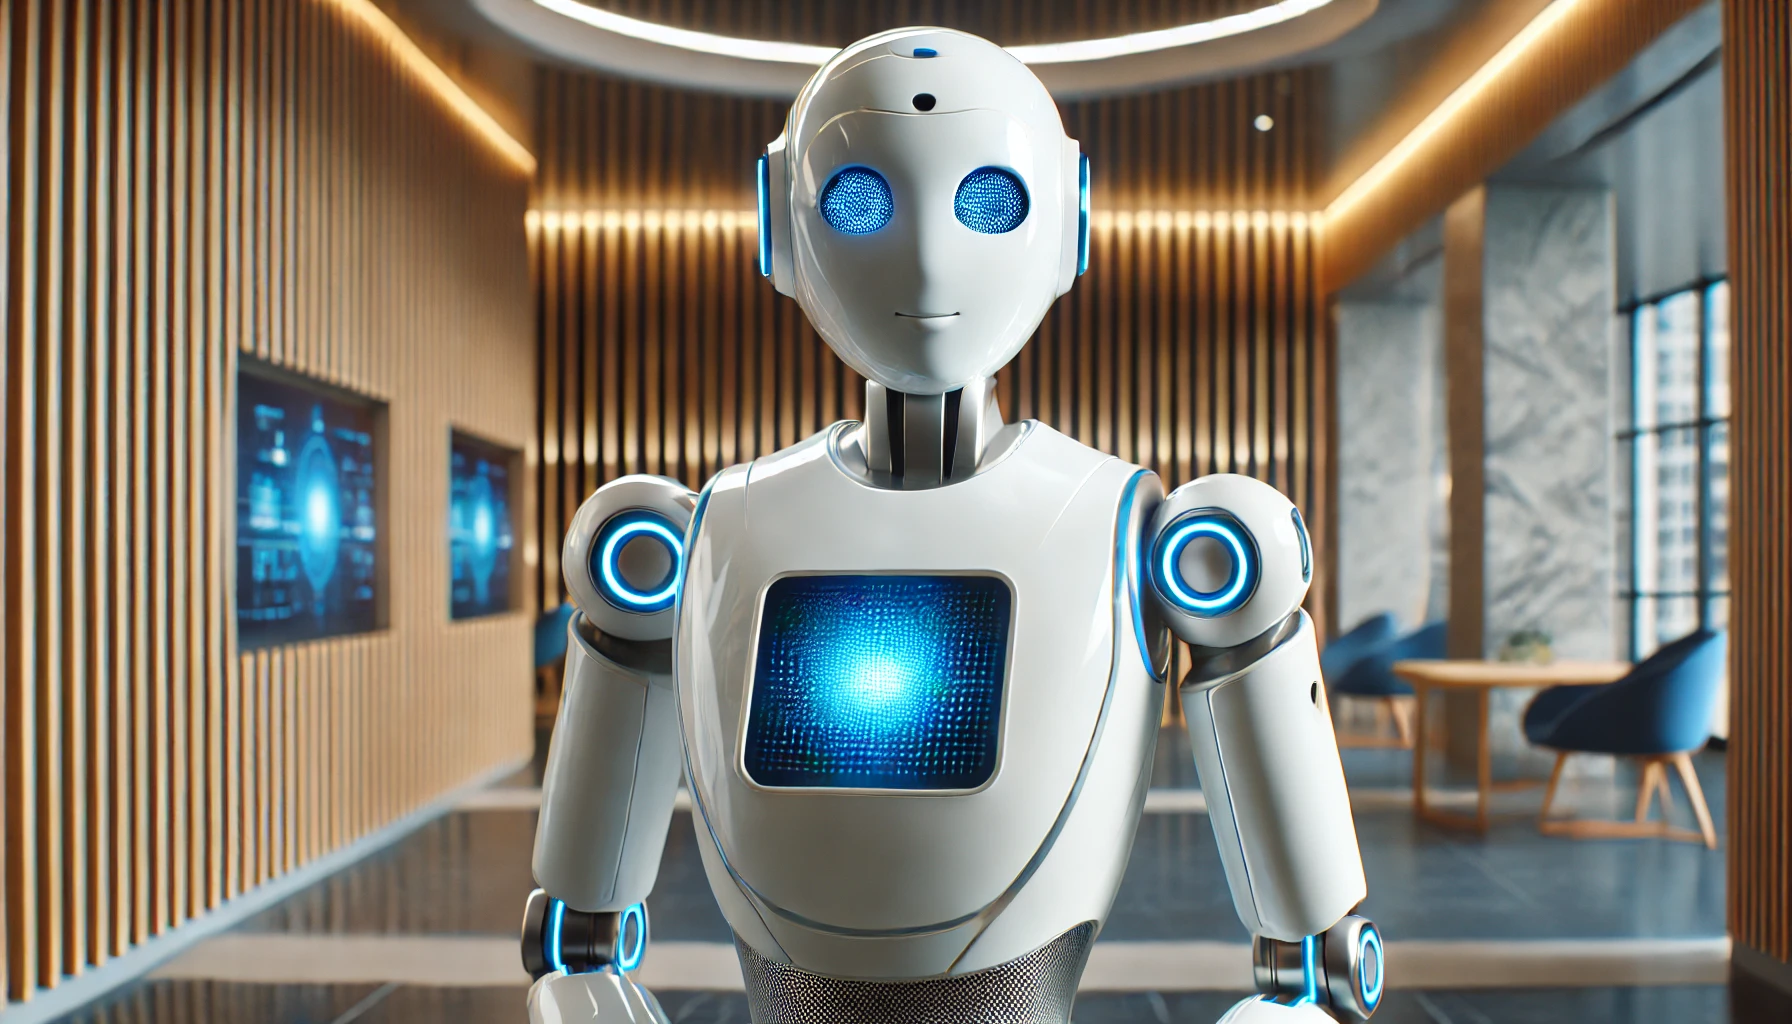
\includegraphics[width=\linewidth]{image/4/AI agent 仿生人.png}
  \caption{智能助手为我们的生活带来便利}
  \label{fig:my_label}
\end{figure}

在这一节中，我们将深入探讨智能助手在不同领域中的应用，特别是在学习、工作和创意产业中的重要作用。首先，我们将探讨智能助手在学习工作中的应用，尤其是如何帮助人们提高生产力、整理任务和优化工作流程。其次，我们将转向人工智能在创意产业的应用，了解AI如何激发创作灵感、推动艺术创作和创新设计的进步。最后，我们将展望智能助手的发展趋势，探讨未来技术如何进一步提升智能助手的能力，使其更加智能化、个性化和情境化，成为更加精准和高效的助手。

这一节将为读者提供全面的视角，展示人工智能在实际生活中的广泛应用，帮助我们更好地理解这一技术如何不断改变我们的工作和生活方式。

\subsection{AI Agent}

AI Agent，你或许已经听说过。很多人将它赞美为这一波 AI 热潮的终极形态，也有人认为，这可能是普通人难得可以亲身参与的机会，甚至是最有可能通往 AGI 的道路。那么，AI Agent 究竟是什么？它为何能享有如此高的赞誉？本小节内容，我们将结合一个生动的案例，用最简洁的语言为你梳理其中的奥妙。

\begin{figure}[ht]
  \centering
  \includegraphics[width=\linewidth]{image/4/咖啡馆老板2.png}
  \caption{人类解决问题的过程}
  \label{fig:my_label}
\end{figure}

举个例子，假如你是一家咖啡店的店主。你平时最常思考的问题之一，也许就是“最近该推出什么新品咖啡”或“该怎么改进店里的菜单”。要是你直接把这些问题抛给大语言模型，多半会得到一堆看起来挺有道理，但放到现实中又不太管用的建议。对于这种知识密集型、需要多方考量的决策任务，仅靠与大语言模型的一次简单对话，几乎无法得到真正有价值的结果。
我们不妨先来看看人类自己是怎么解决这类问题的。通常，我们会先列出一些影响咖啡销量或口味选择的重要因素，比如天气冷热、顾客喜好趋势、原材料成本、门店空间和设备能力等等。然后，自然而然地把宏大的目标拆分成几个更容易执行的小目标，比如，去搜集近期的咖啡市场行情和口味流行趋势；去查看一周或一个月的天气情况，判断是否适合主推冷萃还是热饮；或者去统计顾客对不同产地咖啡豆的偏好。

“目标拆分” 是人类解决问题的惯用思路。接下来，每个小目标都对应具体的动作。例如，先打开天气预报软件，看看未来两周的气温。如果发现气温将大幅回暖，就把新品的重点放到冷饮咖啡上。随后，你可能去各大美食论坛或社交平台，查看人们对冷萃咖啡或特殊口味咖啡（比如椰香、花香）的讨论度和接受度。然后发现最近流行的咖啡配料是“燕麦奶 + 盐味焦糖”，于是你又会进一步聚焦这个方向。

再来，你打开电商网站或咖啡豆批发平台，看看哪些品牌的燕麦奶好评高、成本合适，又或者留意哪个焦糖口味的销量好、口感评价正面。这样反复搜集信息、尝试计算成本后，你也许就能得出一个比较理想的新品思路。假如成本太高，就要再次“碎碎念”，回到“除了盐味焦糖，还有没有性价比更高、容易引爆社交媒体话题的口味”这个思考路径上。

在这个过程中，你会发现，人类在解决复杂问题时，往往陷入一种“思维碎碎念”的状态（我们称之为“思维链”）：在这个“思维碎碎念”的过程中，我们总会情不自禁的将一个复杂的大目标拆分成许多更好解决的小目标，然后一步一步的去逐个击破，并且我们每次还会根据动作产生的结果，对小目标的分解进行调整，然后继续实施不断重复这个过程，直到越来越接近或者说收敛到初始目标的答案。

\textbf{1.AI Agent：模仿人类“思维碎碎念”的尝试}

AI Agent 正是人们在大语言模型的基础上，模拟人类这套思考与行动过程的一个尝试。所谓 Agent，虽然主流的翻译是“智能体”，但笔者更倾向于它的本意——“代理”，也就是让 AI 代理人类去完成这套不断思考、拆分目标、执行动作并回收结果的循环。

\begin{figure}[htbp]
  \centering
  \includegraphics[width=\linewidth]{image/4/AI agent 仿照人类的思维模式.png}
  \caption{AI Agent模仿人类思考过程}
  \label{fig:my_label}
\end{figure}

回到这个“咖啡店新品决策”的问题。在 Agent 的系统中，大语言模型就相当于“人类的大脑”。不过，我们给模型的提示词（Prompt）会比简单的问答要复杂得多：

首先，我们告诉模型“你是咖啡店店主”，并设定它的目标——“要推出最受顾客欢迎的新口味咖啡”。

接着，我们还会告诉它：在这个过程中，人类会用到各种各样的工具，比如上网搜索、数据统计、配方计算、社交平台监测等。因此，在 Agent 系统里还会有一个工具模块，预先编写了网络访问接口、数值计算接口，甚至可运行 Python 代码的环境，以及文件读取、数据库访问等功能。

最后，我们会要求模型在输出结果时，必须严格遵循特定的格式：例如，先输出一段思考推理，再给出目标拆分结果，最后明确当前要执行的动作。

这就是 AI Agent 系统中的“计划”和“动作”模块。当我们把精心设计好的提示词输入到模型后，模型会先给出一段推理，说明“我想要查看天气情况，了解近期冷饮需求趋势”，然后拆分出小目标（比如“去查看天气”“去查社交媒体口味偏好”），再给出当前需要执行的动作（比如“查询天气接口”）。因为我们对回复格式有严格限制，就可以用程序自动地解析出哪个动作应该被执行，然后去调用对应的工具接口。

一旦工具接口给出了结果，我们再把这个结果插入新的提示词里发给模型。模型会根据新的信息，进一步推理、给出新的目标拆分与下一步动作。如此循环往复，这个“机器碎碎念”的齿轮就开始源源不断地转动，模仿人类的思考过程，逐步逼近一个可行的最终答案。

% \begin{figure}[htbp]
%   \centering
%   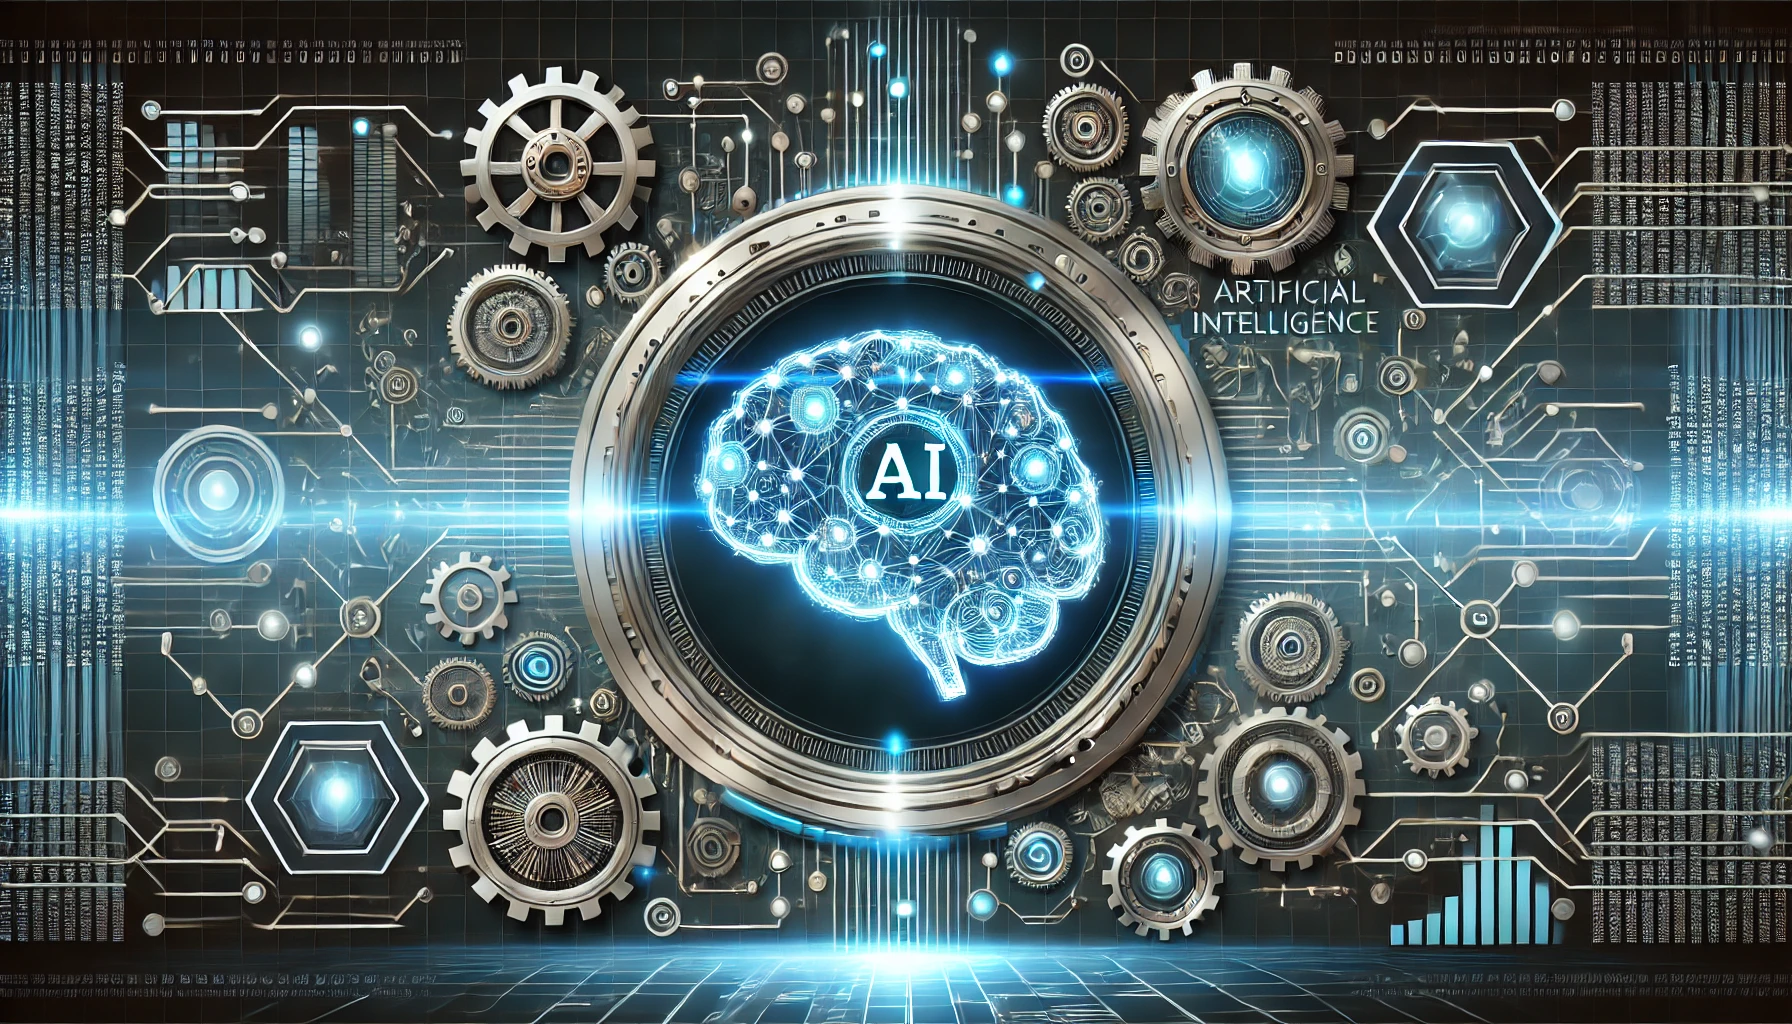
\includegraphics[width=\linewidth]{image/4/AI与齿轮.png}
%   \caption{Caption}
%   \label{fig:my_label}
% \end{figure}

需要注意的是，每一轮模型和工具之间的互动，都产生了很多上下文信息，比如先前的推理内容、目标拆分思路、工具返回的数据等。因此，Agent 系统里通常还会包含一个“记忆模块”，用来记录和管理在对话过程或工具执行过程中产生的各种信息（文本、文件、数据等），以便在后续步骤里再次调用。

\textbf{2.为什么大家如此看好 AI Agent？}

AI Agent 近乎完整地模拟了人类在解决复杂问题时的思考方式和工具使用行为。因此，许多人相信这是一种极可能实现 AGI 的路径。而且，除了用“大语言模型”作为“大脑”以外，这套系统的其他模块——比如网络搜索、数据库管理、数值计算等——都是我们常见的工程技术。普通人只要花些心思学习和调试，也能搭建一个初步的 Agent 系统。

% \begin{figure}[htbp]
%   \centering
%   
\includegraphics[width=\linewidth]{image/4/AI Agent.png}
%   \caption{Caption}
%   \label{fig:my_label}
% \end{figure}

这意味着，在大模型时代，普通人也有机会参与其中，通过创意的提示设计、工具整合、功能调优等手段，做出一个让人眼前一亮的 Agent，并在商业上取得一定的成功。


\textbf{3.AI Agent 的现实问题与挑战}

当然，也有不少反对者认为，AI Agent 目前还不够成熟，只不过是一个极具梦幻色彩的泡沫罢了。它建立在一个前提之上：大语言模型的推理能力要接近甚至匹配人脑，但以现在的模型性能来看，距离真正的“通用智能”还相去甚远。可能在演示时，Agent 的思考过程看似完美；但在现实中，如果运行十次，往往只有少数几次能产出真正富有洞察力的结果。

因此，AI Agent 目前总体属于“理想极其美好、现实尤为严峻”的状态。它既引人期待，又有很多问题亟待解决，比如：1）大语言模型的知识盲区和幻觉（Hallucination）；2）工具调用的异常和错误；3）提示词的安全性与保密性；3）系统运行的性能和成本等等。

% \newpage
\subsection{AI与艺术}
人工智能在过去被认为最难被机器替代的艺术领域，早已闯出一片新天地。人工智能，作为尚未公认的第十艺术，其通用性早已平行于已有的传统八大艺术，甚至有了与新兴的第九艺术——游戏——并列的可能。传统的八大艺术包括文学、音乐、舞蹈、雕塑、绘画、建筑、戏剧、电影八种艺术门类，而尚未获得公认的第九艺术，即是当代青少年所推崇的新兴艺术形式——游戏，某些地区则认为是漫画。

\begin{figure}[ht]
  \centering
  
\includegraphics[width=\linewidth]{image/4/AI 绘画蜂鸟.png}
  \caption{AI绘制出的蜂鸟采蜜图}
  \label{fig:my_label}
\end{figure}

\textbf{1.AI 的“日常艺术”渗透}

秉持实用主义的人工智能，能够跻身艺术这一领域，人们或多或少会觉得有些意外。但笔者认为，现如今，日常生活中，人们已经离不开人工智能的陪伴。举些身边的例子：AI哭脸算法。过去几周，TikTok上出现了无数哭脸滤镜的短视频，被拍的人再怎么努力大笑，镜头里依然是满眼含泪、苦大仇深的样子。无论是肌肉壮汉、优雅小姐姐，还是可爱小朋友，入镜后都变成了伤透心的模样。由于太过魔性，这个滤镜迅速引发了一场用户间的恶搞狂欢。

AI马赛克消除算法则通过将一张图片随机遮挡，利用AI算法进行复原。尽管算法调校依然是散漫的，但它依然能够真实还原图像。传统的去马赛克方法是通过填充像素邻近点，而使用Pulse技术的Face Depixelizer，则通过从AI图像库中找到较接近的图像，进行高清图像与马赛克图的合成，最终生成更清晰的图像。比如，它能把16x16的像素图放大到1024x1024高分辨率。

% \begin{figure}[ht]
%   \centering
%   
\includegraphics[width=\linewidth]{image/4/AI去马赛克.png}
%   \caption{使用CodeFormer工具图片清晰化前后对比}
%   \label{fig:my_label}
% \end{figure}

\begin{figure}[ht]
  \centering
  
\includegraphics[width=\linewidth]{image/4/人脸清晰化.png}
  \caption{使用CodeFormer工具人脸清晰化前后对比}
  \label{fig:my_label}
\end{figure}

接着是AI原神自动钓鱼算法，想必各位热衷二次元的小伙伴们都知道，游戏中有个钓鱼玩法。这个算法分为两个部分：鱼群定位与识别，拉杆时机的计算策略。在抛杆时，使用目标检测的UX算法，拉杆时机则采用强化学习的DQN算法，这与魔兽世界中的钓鱼脚本效果大致相同。

AI声音模仿算法则能在5秒内克隆你的声音。只需录制一段5秒左右的声音，AI算法就可以根据这段音频生成你事先输入的文字对应的合成音。

AI二次元全身生成算法，与其他类型不同的是，它可以生成整个身体，算法基于GAN实现。这个算法满足了玩家们组建二次元后宫的梦想。

除此之外，还有老照片修复、图片生成视频、AI换脸、文生视频等等一系列新的AI玩法正悄然渗透到我们的日常生活中。这些渗透到日常生活中的实用主义人工智能，正在悄悄地改变我们的生活习惯，而大众的审美也在人工智能的干涉下悄悄发生变化。

\textbf{2.AI艺术的崛起与关键事件}

人工智能在艺术领域，已由悄悄发力转变为开足马力了。时间回溯到2016年，谷歌刚刚嗅到了人工智能在艺术领域的商机，并发布了品红计划，试图让机器学会自主合成艺术与音乐。随后，人工智能艺术在全球科技巨头的努力下，开始井喷式增长。

\begin{figure}[ht]
  \centering
  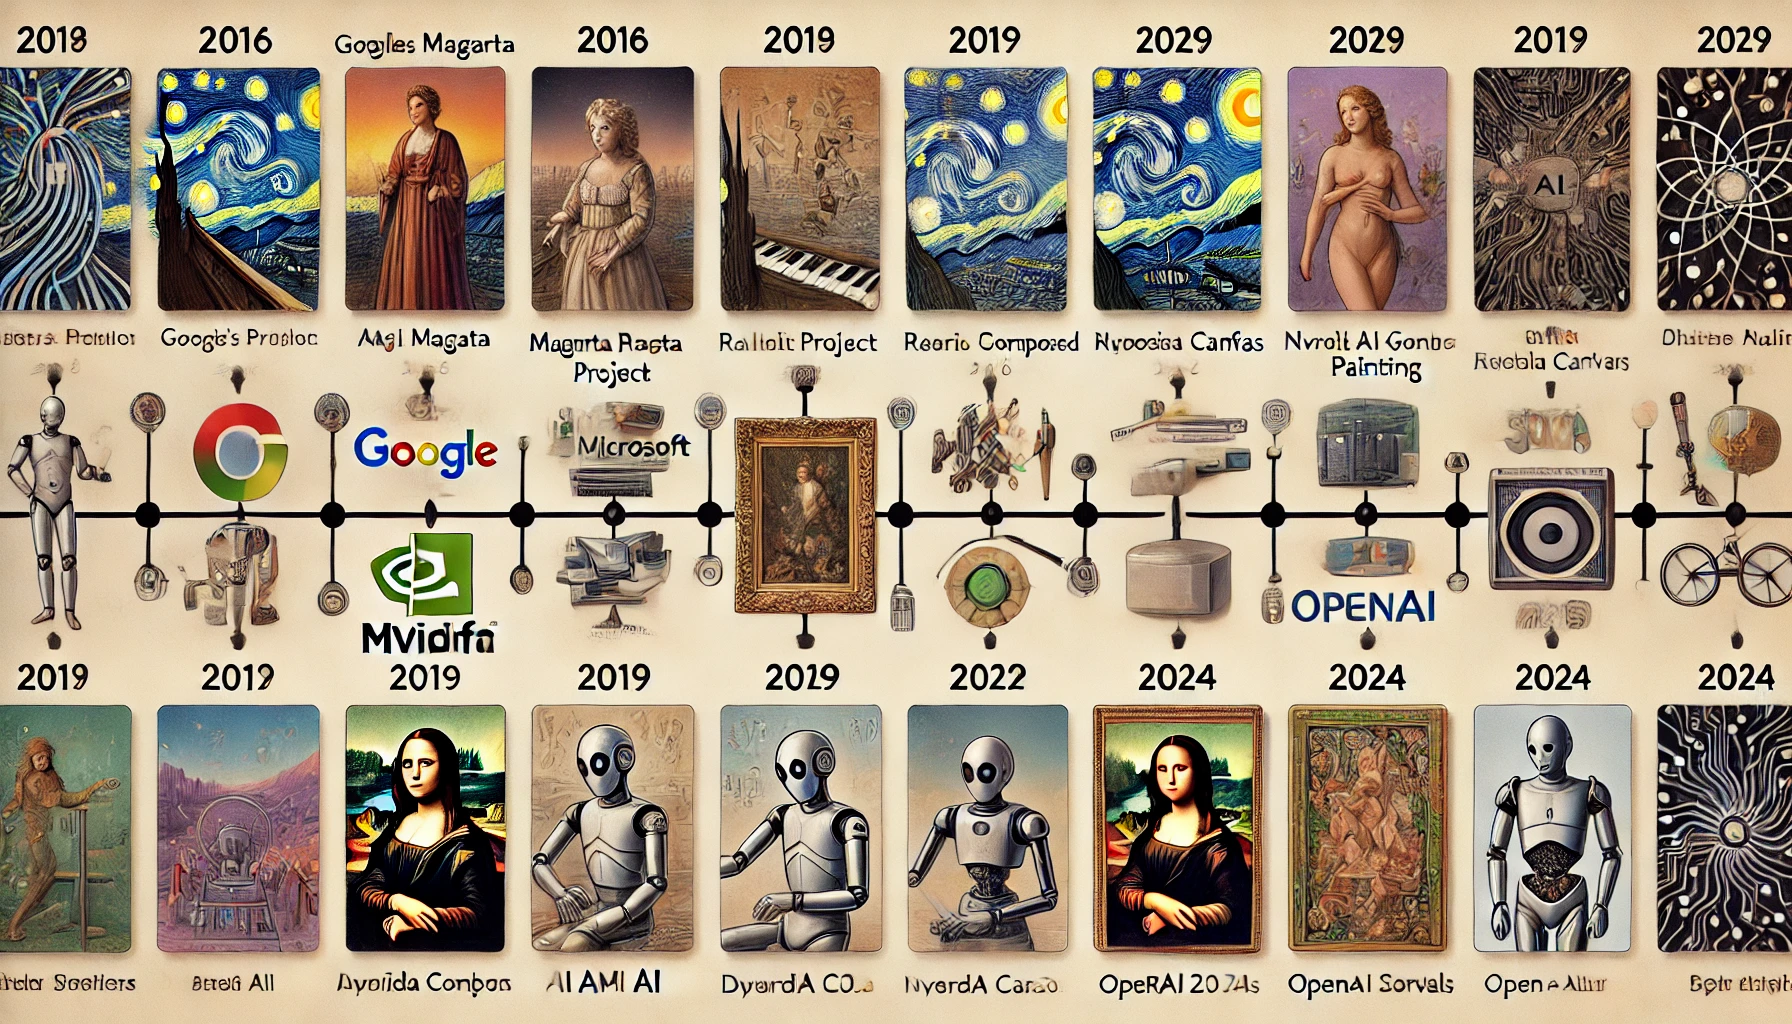
\includegraphics[width=\linewidth]{image/4/ai发展时间轴.png}
  \caption{Caption(待优化)}
  \label{fig:my_label}
\end{figure}

2016年4月，微软与荷兰国际集团联合研发的机器学习系统成功复制了伦勃朗的经典画作。2017年8月，Tarron的新专辑《I Am AI》中，第一首推出的歌曲《Breaking Free》，是由一个名为Amper的人工智能负责作曲和监制的。这是全球首张人工智能作曲和制作的专辑。2017年10月，阿里AI鹿班上岗，每秒可以制作8000张海报，使得艺术界，尤其是设计界为之疯狂。

2019年10月，首次使用人工智能创作的艺术作品《爱德蒙·德·贝拉米肖像》，在纽约嘉士德被拍卖，并最终以35万美元的价格成交。那时，人工智能已经在艺术领域展露头角。然而，谁也想不到，颠覆艺术创作领域的大事件就在不久的将来发生了。

2021年，一个闪光弹照亮了AI艺术领域不那么明亮的夜空——DALL·E问世了。发布首日，官网流量瞬间爆棚。功能上，DALL·E可以根据用户的关键词生成富有创作性的艺术作品，出色的表现让它在AI圈中刷爆了热度。开发团队也没闲着，2022年4月，OpenAI发布了DALL·E 2.0版本。该版本不仅可以像1.0版本一样从自然语言的描述中创建逼真的图像和艺术，还可以对现有的生成图片进行二次创作。它能够根据文本描述中的概念、属性和风格等三个元素进行系统的排列组合，生成任意风格的图像与艺术作品。分辨率也提高了4倍。

在艺术上，DALL·E是基于文图对照的训练方法，与传统的纯图片数据集或纯文本数据集不同。DALL·E结合了两者的特点，就像一个N维数组，经过N个图像特征与N个文本集合的两两比对。比对结果并不像传统的机器学习一样追求高匹配度，而是追求做出大体类别的分类。输出结果是基于真实文本描述与图像特征的对比，最终解码生成图片。

一些脑洞惊奇的用户们，通过DALL·E这个工具，分享出了自己对这个世界的独特理解。这些作品与车尔尼·雪夫斯基在《艺术对现实的审美关系》中提到的“艺术来源于生活，却又高于生活”的观点相呼应。普通人没有艺术家灵魂，无法像画家一样利用乐器展现自己，表达思想。而DALL·E作为一种人工智能的通用能力，给那些没有涉足过艺术领域的普通人，提供了一种展示自己想法与观点的途径。

与DALL·E颇具创造性的特点相似的同类产品NVIDIA Canvas，也为热爱创作的普通人提供了一种创作的新途径。你只需在画布上画出简单的涂鸦，AI就会实时将其转化为栩栩如生的艺术作品。该工具一经面世，便在全球各大展会上引起了创作群体的轰动。在此基础上，NVIDIA Canvas允许创作者使用素材而非色彩进行创作，AI将简单的笔触转化为栩栩如生的画作，甚至可以使用现实世界中的草、云、山、水等素材来创作。AI模型会在显示屏上展现出写实的结果。

OpenAI于2024年2月15日向公众展示了由Sora生成的多个高清视频，称该模型能够生成长达一分钟的视频。同时，OpenAI也承认了该技术的一些缺点，包括在模拟复杂物理现象方面的困难。《麻省理工科技评论》的报道称演示视频令人印象深刻，但指出它们可能是经精心挑选的，并不一定能代表Sora生成视频的普遍水准。

2024年12月9日晚，OpenAI正式向ChatGPT Plus和ChatGPT Pro用户公开发布Sora的试用版本，这些付费用户可以开始使用Sora。Sora的诞生，开启了文生视频的新纪元。

\textbf{3.从二维到三维的进阶}

阅读完上文，人工智能输出2D艺术作品已经是天花板了吗？并不是的，技术还有更多进展。在动画与游戏制作领域，三维旋转技术已经具备了成熟的技术方案。传统的二次元游戏已经将这一技术运用得炉火纯青。可是，给出2D图像后，进行三维逆操作，你见过吗？q Blocks团队给出了这样的研究成果。团队成员通过超大数据集训练，将物理表象渲染的3D建模新技术推送到大家面前。该技术为恢复完整的3D建模提供了成熟的解决方案，可以说是一种真升维打击。尤其是对于二维图像中复杂的特征点形状交织问题，具有很好的处理效果。感兴趣的同学可以阅读文末的这篇论文。[qblocks相关论文]
% (http://rgl.s3.eu-central-1.amazonaws.com/media/papers/Vicini2022sdf_1.pdf)

\begin{figure}[ht]
  \centering
  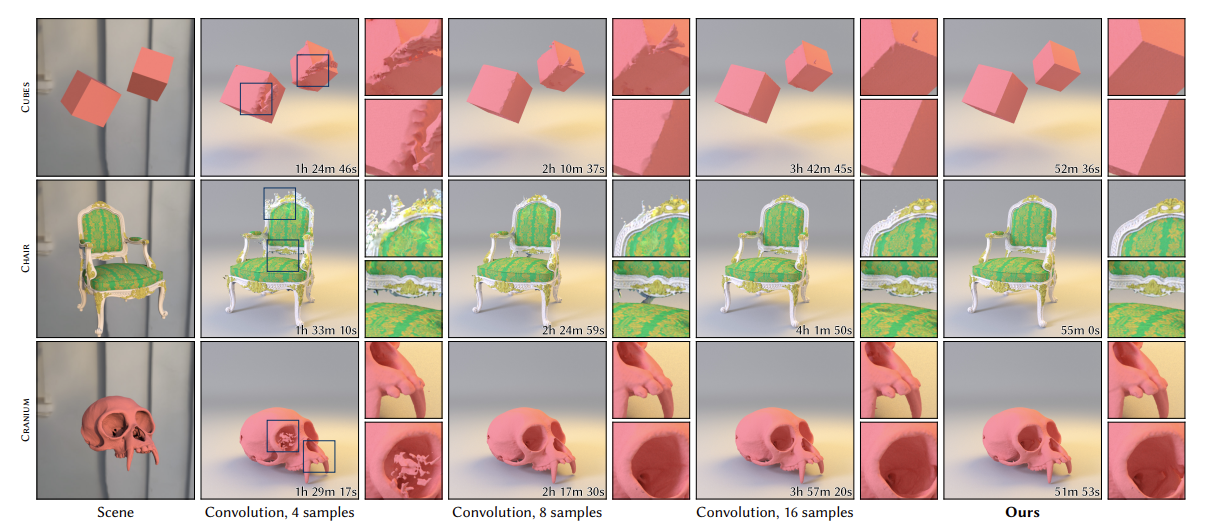
\includegraphics[width=\linewidth]{image/4/2D-3D.png}
  \caption{q Blocks 团队实现2D到3D的跨越}
  \label{fig:my_label}
\end{figure}

\textbf{4.AI 艺术：创意无疆，未来可期}

总的来说，AI艺术创作的背后，神经网络（GNN）起到了支撑作用。在生成图像的训练过程中，GNN可以将真实世界的物体模型转化为真实图像，艺术家则可以对其进行再训练，识别新的模式并创造无限可能。尽管有边界的数据集可能让创意暂时受限，但随着技术的进步，边界将会逐渐弱化，传统艺术形式也会被注入更多的灵感与创意，让人们不再感受到技术壁垒，文化边界的阻隔。创意会随时随地展示给他人，真正做到“源于生活，高于生活”的艺术。

人工智能正在人类最不可替代的领域大放异彩的同时，普通人如何参与其中并获得自己的收获呢？谷歌的工程总监雷·库兹维尔在对未来的预期中，一直拥有独到的眼光。他提出，技术奇点将在未来30年的某个时间点出现，我们会好奇这个奇点会以何种形式出现呢？他认为，这一奇点的到来，将让人类拥有接近10亿倍的智力提升，并能通过计算机将大脑与云端连接，打开思维的新边界。这种看似遥不可及的愿景，早在人工智能成为热点技术的今天，早已不再是一种遥远的幻想。

国内一些领先的AI公司（如地平线、商汤科技、Momenta等）在业务拓展上，已经准备好迎接人才的加入。如果有志于进入这个行业，也不必害怕知识的落后，始终保持热情，不断学习，掌握算法开发、前后端开发等技能，你就能够为自己的未来打开一扇窗。

人工智能的进步远不止于此，它将带来更多的可能与挑战。机器不断进步的同时，如何与人类共生，将是人工智能发展的关键之一。而艺术的边界正在不断被打破，人工智能与人类的创造力，也将在共同推动下，带领这个世界走向更美好的未来。

% \newpage
\section{智能交通}

随着城市化进程的加快和科技的发展，传统交通系统面临着越来越多的挑战，包括交通拥堵、交通事故频发和环境污染等问题。在这种背景下，智能交通应运而生，成为解决这些问题的关键技术之一。智能交通不仅利用人工智能、物联网、大数据等技术手段提升交通管理效率，还通过自动驾驶和智能车载系统等创新应用，极大地改善了交通流动性、降低了事故率，并推动了交通领域的革命性变革。

在本节中，我们将重点探讨智能交通的几大核心应用，首先分析自动驾驶与智能车载系统如何通过人工智能技术实现车辆的自主驾驶，并带来更安全、更高效的出行方式；接着探讨智能交通管理与优化，了解如何通过数据分析和实时监控系统优化交通流量，缓解拥堵并减少环境污染。

通过本节内容，读者将全面了解智能交通技术如何在提升交通安全、减少能源消耗、优化出行体验等方面发挥重要作用，同时也能预见到这一技术在未来城市交通系统中的巨大影响。

\begin{figure}[ht]
  \centering
  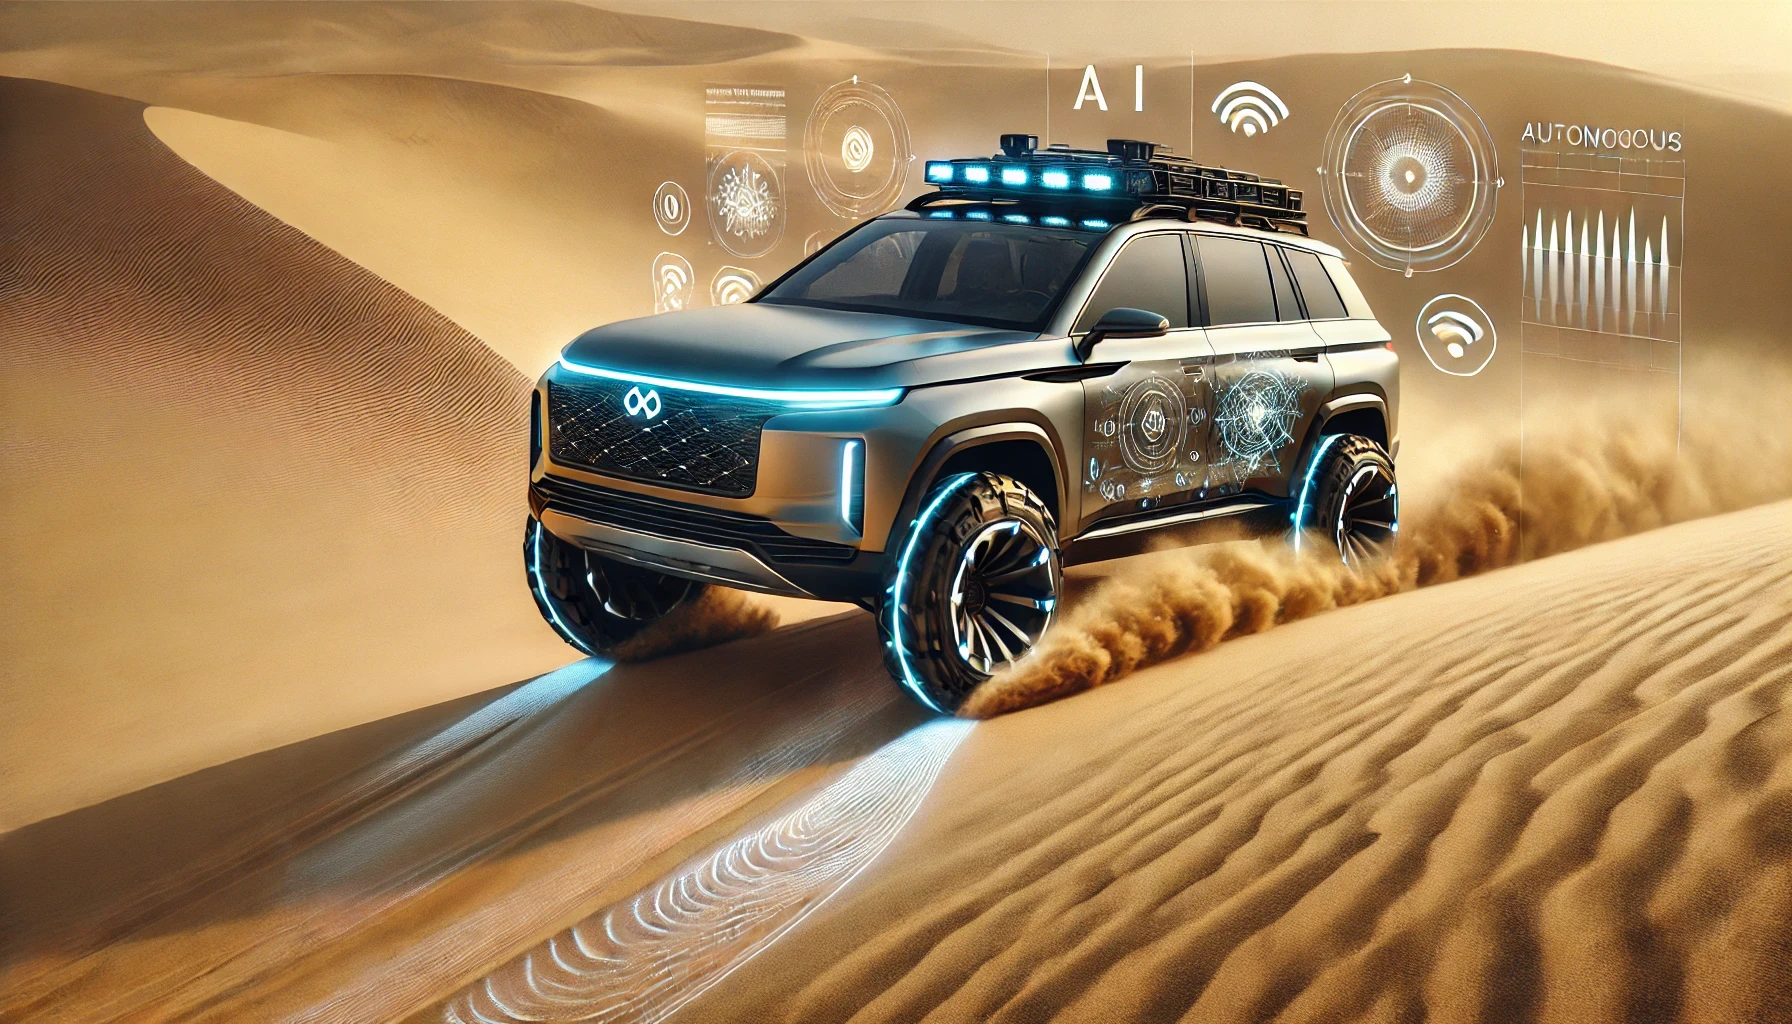
\includegraphics[width=\linewidth]{image/4/AI沙漠汽车.png}
  \caption{自动驾驶概念车行驶在沙漠中}
  \label{fig:my_label}
\end{figure}

\subsection{自动驾驶}



20年前，大洋彼岸的美利坚设置了百万赏金，策划了一场关于自动驾驶的挑战赛。最终，获胜的选手仅仅是在沙漠中行驶了10公里就赢得了100万美元的奖金。这看似轻松的胜利，可能更多地考验了选手的胆量和运气。然而，这场比赛之后，自动驾驶技术开始进入公众的视野，人类对其认知也从那时起逐步提升。随着技术的不断进步，自动驾驶进入了一个缓慢而持续发展的历史时期。回顾今天，自动驾驶的发展可以用“缓慢且坚定”来形容，充满了浪漫色彩。

\textbf{1.自动驾驶辅助“为什么贵了好几万？”}

谈到自动驾驶，首先会听到一大串英文缩写，比如 ACC、LCC、MGP、NOA 等等。有人好奇：这些功能到底能干什么？车价为何会因此多出 5～6 万元？随着拥有这些功能的车型日渐增多，这些配置也逐渐成为许多消费者选购汽车时的“刚需”。但若对其原理和等级划分并不熟悉，就很容易被各种宣传名词搞得一头雾水。

\textbf{2.SAE 分级：从 L0 到 L5}

根据 SAE（美国汽车工程师学会）的通用标准，自动驾驶从 L0 到 L5 共分 6 个级别，各级别大致如下：
\textbf{L0（无辅助）}：纯人工驾驶，不具备任何自动化功能。很多入门车型依旧停留在这一等级。
\textbf{L1（单项辅助）}：车辆在方向盘\emph{或}车速中有一项由系统控制，另一项仍由驾驶员负责。最常见的例子是“定速巡航”或基础版“ACC 自适应巡航”。
\textbf{L2（多项组合）}：车辆在方向盘和加减速两方面都有辅助功能。ACC + 车道保持（LCC）是典型组合，能够在车道内自动跟车并保持方向，但仍需驾驶员全程集中注意力。
\textbf{L3（有条件自动驾驶）}：在特定环境下，车辆可完成绝大部分动态驾驶任务，驾驶员可暂时“脱手、脱脚”，但必须保持随时接管的准备。
\textbf{L4（高度自动驾驶）}：几乎所有驾驶动作都能由系统完成，驾驶员在绝大多数情况下可以不管方向盘。部分城市无人出租车项目（“萝卜快跑”等）大致接近这一等级。
\textbf{L5（完全自动驾驶）}：车辆在任何场景都能独立驾驶，人类仅仅是“乘客”。这是自动驾驶的终极形态，尚不知何时能全面实现。

\begin{figure}[ht]
  \centering
  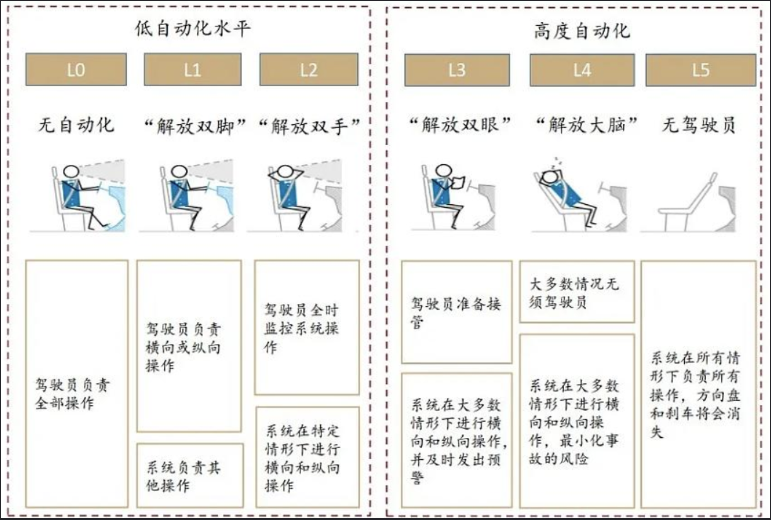
\includegraphics[width=1\linewidth]{image/4/SAE 分级.png}
  \caption{SAE 分级示意图（待优化）}
  \label{fig:my_label}
\end{figure}

\textbf{3.探索“NOA”与“端到端”大模型}

在目前市售车型中，NOA（Navigation On AutoPilot，导航辅助驾驶）功能尤为吸睛。它可在高速或城市道路上，按照预先设置的导航路线实现自动变道、超车、进出匝道等操作，一定程度上接近 L3 标准。因为需要更多高算力芯片、激光雷达等硬件，带有 NOA 的车型通常更昂贵。不同品牌的汽车厂商会根据各自的市场定位和技术特点，为 NOA（导航辅助驾驶）功能取不同的名称，但其核心功能本质上是相似的，主要实现自动变道、进出匝道、路径规划等操作。例如：小鹏汽车将 NOA 命名为 XNGP（Xiaopeng Navigation Guided Pilot），功能覆盖高速、城市路况及停车场等复杂场景，定位于“全场景智能驾驶”。华为在其智能驾驶解决方案中，将 NOA 称为 NCA（Navigation Cruise Assist），主打城市道路的导航辅助，已应用于部分搭载华为智能座舱的车型（如赛力斯华为智选 SF5）。蔚来（NIO）将 NOA 命名为 NOP（Navigate on Pilot），主要用于高速导航辅助，搭载于 NIO Pilot 系统中，可实现自动变道、匝道行驶等功能。理想汽车其 NOA 功能被称为 AD Pro（Advanced Driver Pro），强调在高速路和城区多场景下的自动驾驶体验。特斯拉的 NOA 名为 Navigate on Autopilot，包含在其 Autopilot 高级辅助驾驶包中，支持高速路自动驾驶辅助和智能导航功能。比亚迪的高阶辅助驾驶功能名为 DiPilot，包含城市导航辅助驾驶和高速 NOA 等模块。

虽然名称不同，但这些功能的核心都是围绕导航自动化展开，通过摄像头、毫米波雷达、激光雷达等多模传感器协同工作，结合高算力芯片和算法实现对路径的实时决策和动态调整。随着技术的逐步发展，不同品牌的 NOA 功能差异也会逐渐缩小，但细节体验仍有赖于车企的调校和技术优化。

近来，主打“端到端大模型”的厂商也不断涌现。所谓“端到端”，是指用更先进的 AI 算法，让车辆像人一样对复杂路况进行实时分析与决策，并在行驶过程中及时应对突发状况。它对算力要求更高，随着技术迭代，这类方案将变得愈发可靠。

\textbf{4.自动驾驶走进日常生活}

随着技术加速发展，各种无人配送车、无人驾驶出租车、无人巴士等正在陆续走进我们的视野。通过环境感知、路径规划以及对车辆的自主控制，自动驾驶被认为能显著提升道路交通安全、缓解拥堵，并带来更便捷的出行体验。

\begin{figure}[ht]
  \centering
  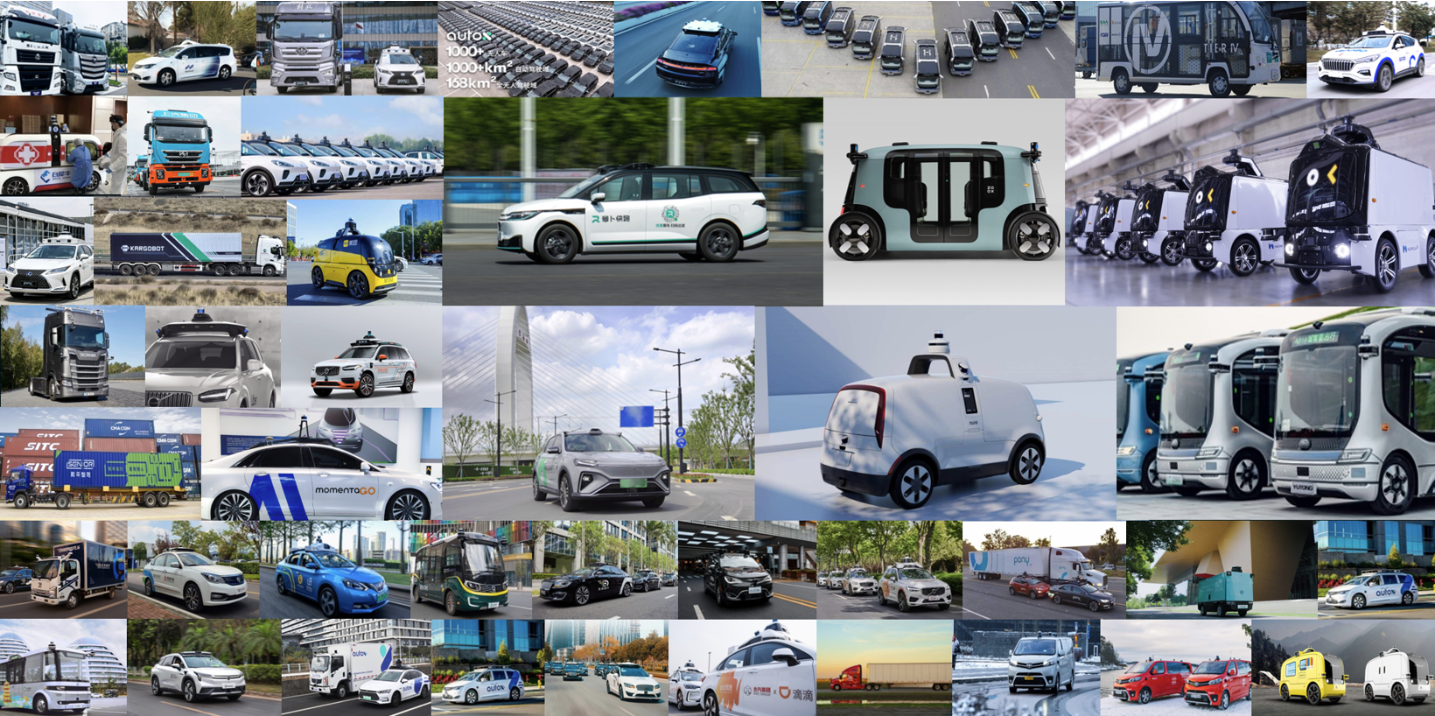
\includegraphics[width=\linewidth]{image/4/日常智能驾驶.png}
  \caption{日常生活中的自动驾驶汽车}
  \label{fig:my_label}
\end{figure}

例如，近段时间百度的“萝卜快跑”项目已在武汉等多个城市落地，提供高度自动化的无人出租车服务。乘客只需通过手机 APP 一键预约，车辆便可实现从接驾到目的地的一整套全自动驾驶服务。虽然目前仍需配备安全员以应对突发情况，但这一模式的推广，已经让人们对未来的完全自动驾驶场景充满期待。

与此同时，车联网（V2X）技术也在加速完善。车辆与基础设施（V2I）、车辆与车辆（V2V）、车辆与行人（V2P）等多种交互形态，让汽车与周围环境时刻保持数据通信。配合智能交通信号系统、实时路况分析以及 5G 网络，自动驾驶的落地性和安全性将逐步提升。

\textbf{5.面向未来：人机交互的下一站}

虽然 L5 级完全自动驾驶仍是未来愿景，但从 L2-L3-L4 的持续迭代中，我们已窥见了技术的潜力。高算力芯片、激光雷达、多模传感器以及端到端 AI 模型的结合，都为自动驾驶铺平了道路。

 毫无疑问，自动驾驶将是我们未来出行的重要组成部分。技术依旧在进步，法规和社会接受度也将不断演变。人们可以期待，在不远的将来，车辆真的会成为“智能领航员”，为我们的出行带来全新的安全与便捷。

\subsection{智慧交通}

 最近，武汉市的“萝卜快跑”无人驾驶出租车正式上线，引发了市民们的强烈关注。乘客只需通过手机 App 下单，车辆就能实现从接驾到目的地的一整套自动驾驶服务。高峰期时甚至“一车难求”，可见人们对这类“科幻级”出行方式的好奇与认可正与日俱增。

\begin{figure}[ht]
  \centering
  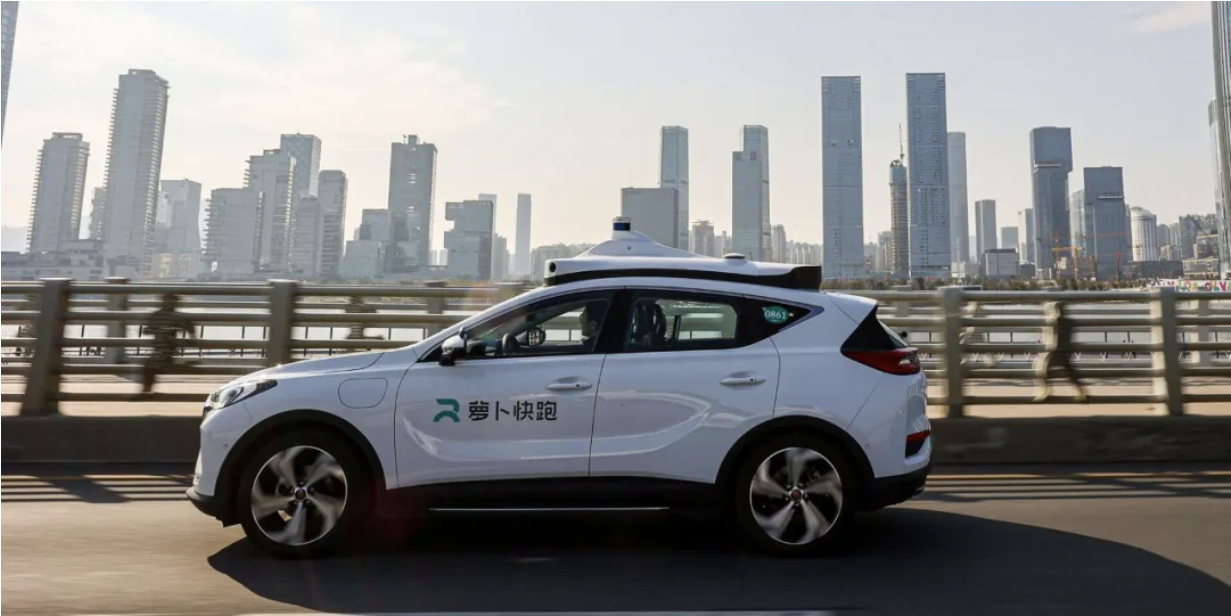
\includegraphics[width=\linewidth]{image/4/robo快跑.png}
  \caption{萝卜快跑汽车行驶在公路上}
  \label{fig:my_label}
\end{figure}

那么，承载智能出行的“智慧交通”系统究竟如何运作？它在技术上是如何实现的？又会给我们的城市与生活方式带来怎样的改变？本节，我们就从“城市大脑”的角度，探讨面向未来的交通变革。

\textbf{1.从“单车智能”到“城市大脑”：智慧交通的核心}

\begin{figure}[ht]
  \centering
  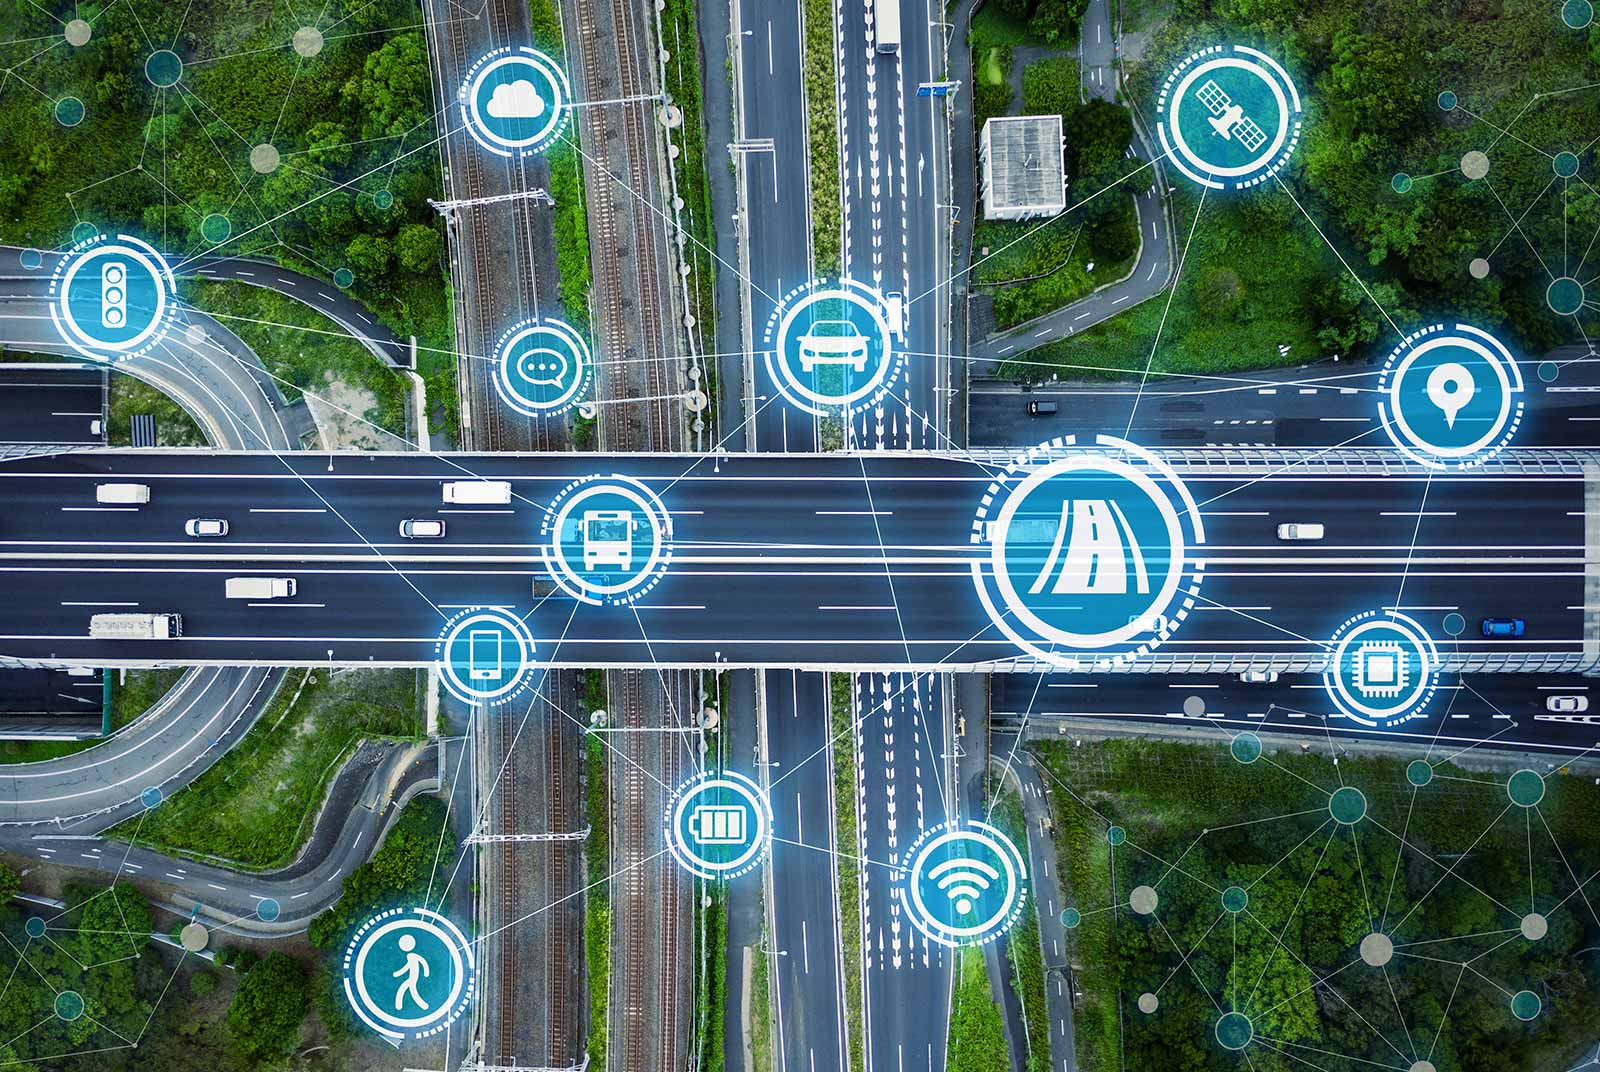
\includegraphics[width=\linewidth]{image/4/智慧交通.jpg}
  \caption{智慧交通万物互联概念图}
  \label{fig:my_label}
\end{figure}

智慧交通是智慧城市建设的重要组成部分，涵盖了无人驾驶、车路协同、交通信号优化、智能泊车以及城市级的宏观调控等诸多领域。与“单车无人驾驶”相比，智慧交通更侧重“全局最优”。单车智能中，每一辆无人车都在追求自身路径规划的最优，通过摄像头、雷达等传感器和算法，自行避障、行驶、并在局部范围内做实时决策。城市大脑将单车运行的所有信息汇总，通过海量的数据分析和运筹学算法，从整体角度对整个城市的交通进行调度、优化和管理。

然而，仅靠单车层面的最优选择，有时会陷入“囚徒困境”，难以实现城市级的畅通。只有在“城市大脑”——这只“看得见的手”的调度下，才能让交通真正走向“全局最优”。

\textbf{2.大数据是“城市大脑”的基石}

智慧交通的前提在于数据的获取、传输与存储。如今，城市各个角落布设了交通摄像头、路侧传感器、5G 基站和车联网（V2X）系统，并与无人车辆、公交、地铁、出租车等构成了庞大的数据网络。1）实时监控：摄像头和雷达可记录每条道路的车辆速度、数量、是否发生事故等。2）移动端数据：市民每天通过打车软件、公交刷卡、导航 App 等“留下”出行轨迹，帮助城市大脑构建“人口流动”大数据库。3）5G 传输：关键数据及时回传到云端，让“城市大脑”做出毫秒级的分析与决策。4）边缘计算：部分视频图像或车辆行驶信息会先在传感器端做初步处理，只将必要的数字化结果上传，以减轻网络带宽与云端压力。

有了这些海量数据，智慧交通才能通过准确的运筹模型，动态分析不同路段的拥堵情况，优化公共交通调度，甚至提前预测出交通瓶颈。

\textbf{3.“城市大脑”如何助力交通优化}

 1. 智能交通信号灯

堵车是现代城市中最让人头痛的问题，而红绿灯往往是造成拥堵的主要因素之一。智慧交通系统会实时监控各路口车流量，通过内置的计算机视觉和大数据预测，动态调整信号灯时长，实现1)按需分配：车流量大的方向延长绿灯时间，车流量少的方向缩短红灯等待；2)公交优先：车路协同技术可自动识别公交车位置和行驶速度，为其“量身定制”更高的通行效率；3)精准预测：结合天气、节假日及历史出行数据，提前制定红绿灯配时方案，降低高峰期路口拥堵。

 2. 智能泊车

许多车主在城市中最头痛的莫过于“停车难”。智慧交通通过监测城市中所有停车场、路边泊位的使用状况，结合车辆行驶轨迹和停车需求，进行全局调配：通过 5G 物联网让车辆在出发前就知道目的地附近的车位可用情况；高阶无人驾驶车辆能在抵达停车场后，直接进行“自寻车位+自动泊车”，免去排队与“人肉找车位”的麻烦。

 3. 城市应急响应

当遇到暴雨、事故或重大活动管制导致道路中断时，智慧交通中的城市大脑会实时监测到路段异常，并迅速调用多车路径规划算法，统筹整个城市的车辆行驶路线，调整红绿灯配时、引导应急通道，让交通秩序尽量维持畅通。例如：在事故发生的第一时间通知附近车辆绕行，协调警务及救护车辆快速抵达现场；在遇到极端天气时，按照实时降雨量或积水状况，动态控制重点路口或桥隧通行，减少交通瘫痪。

\textbf{4.畅想未来：从 L5 无人驾驶到空中飞行器}

\begin{figure}[ht]
  \centering
  \includegraphics[width=\linewidth]{image/4/未来智慧城市.png}
  \caption{未来的智慧城市模型}
  \label{fig:my_label}
\end{figure}
如果说 L2-L3 级的无人驾驶已经开始融入日常，那么 L5 级完全自动驾驶 将会让智慧交通再上一个量级。所有车辆由城市大脑统一调度，车流如同“水流”一样在城市中高效运转；个人购买车辆的需求大幅降低，类似滴滴、Uber、百度车队等无人车公司将提供“随叫随到”的移动服务；甚至，未来或将出现“低噪音、全透明”的空中无人飞行器，进一步提升通勤效率，缓解地面拥堵。

当然，想要实现城市中所有车辆同步“上位”到 L5 并非易事，还需长期的技术积累和法律政策的完善。某些新兴试点城市可能会先行一步，通过搭建全新基础设施、从零到一逐步迭代，以较小的试错成本推进智慧交通系统走向成熟。

武汉“萝卜快跑”的出现，为我们揭示了智慧交通时代已悄然来临。当单车无人驾驶与城市大脑强强联手，我们所经历的交通拥堵、找车位难、应急响应慢等诸多痛点，都有望得到系统性的解决。再加上 5G、云计算、车路协同技术的持续迭代，未来城市将不再需要漫长的红灯等待，也无需担心停车难题，甚至可能迎来“空中飞行器”的科幻场景。

可以预见的是，当人类与 AI 一起设计并运营“未来城市的大脑”，城市出行将被重新定义，真正实现高效、便捷、环保与安全的理想交通。让我们拭目以待，见证智慧交通在城市中大放异彩。

\newpage
\section{智慧医疗}

随着人工智能技术的迅猛发展，医疗行业正经历一场前所未有的变革。传统医疗模式中的诊断、治疗和管理方式逐步向智能化、自动化和个性化转型。人工智能不仅可以帮助医生提高诊疗效率，还能够通过大数据分析、机器学习、深度学习等技术，实现疾病的早期预测、精准治疗和全程健康管理。以个性化医疗为例，基因组学与AI的深度融合使得治疗方案更加精准，能够根据患者的遗传信息、生活方式和环境因素量身定制个性化的医疗方案。同时，智慧医院的建设通过智能导诊系统、智能排班和智能监控等技术优化了医疗流程，提升了医疗服务的效率和质量。此外，医学影像与诊断辅助工具的应用，大大提高了诊断的准确性和速度，帮助医生更早期地发现和治疗疾病。随着智能医疗系统的不断完善和普及，医疗资源的配置更加优化，患者的就医体验显著改善。展望未来，人工智能将在医疗领域发挥更大的作用，推动医疗服务向更加精准、高效和人性化的方向发展，为人类健康保驾护航。
\begin{figure}[ht]
  \centering
  \includegraphics[width=\linewidth]{image/4/智慧医疗总图.png}
  \caption{智慧医疗示意图}
  \label{fig:my_label}
\end{figure}

\subsection{个性化医疗}
个性化医疗开启了全新的医疗时代，其核心在于基因组学的应用。通过对个体的遗传信息、生活方式和环境因素进行全面分析，人工智能（AI）能够为每位患者提供量身定制的医疗方案和治疗手段。具体而言，基因组测序和分析使医生能够了解患者的遗传变异和易感基因，从而预测其可能患上的疾病，提供早期预防和干预的依据。此外，个性化医疗还综合考虑患者的饮食习惯、运动情况和环境暴露等因素，制定出适合的治疗方案。

 \textbf{1.基因组学与AI的结合}

基因组学确实是个性化医疗的基石。通过对患者基因组的深度解析，人工智能（AI）技术能够从海量的基因数据中挖掘出有价值的信息。这一过程不仅能够帮助医生了解个体的遗传背景，还能识别出与特定疾病相关的基因变异，从而实现疾病的早期预防和精准治疗。借助先进的测序技术，基因组学能够快速、准确地解码患者的DNA序列，而人工智能则通过强大的数据处理能力，分析复杂的基因网络和表达模式，揭示潜在的生物标志物和治疗靶点。

\begin{figure}[ht]
  \centering
  \includegraphics[width=\linewidth]{image/4/AI基因组学.png}
  \caption{基因组学与 AI 的结合}
  \label{fig:my_label}
\end{figure}

例如，华大基因（BGI）作为中国领先的基因组学企业，已经在多个个性化医疗项目中应用AI技术。华大基因利用其强大的基因测序能力，结合AI算法，为癌症患者提供精准的基因检测服务，帮助医生制定个性化的治疗方案。通过分析患者的基因突变，华大基因能够预测肿瘤的生长趋势和对特定药物的敏感性，从而提高治疗的有效性和安全性。

在癌症治疗领域，个性化医疗通过结合基于影像组学和人工智能（AI）的先进技术，显著提升了临床决策的精准性和有效性。利用AI驱动的影像生物标记物，医生能够从患者的常规医学影像（如CT、MRI和PET扫描）中提取丰富的定量特征，深入分析肿瘤的形态、纹理及其微环境。这些特征不仅有助于准确预测疾病的预后，还能够评估患者对各种治疗方案（包括化疗、放疗、靶向治疗和免疫疗法）的潜在反应。

\begin{figure}[ht]
  \centering
  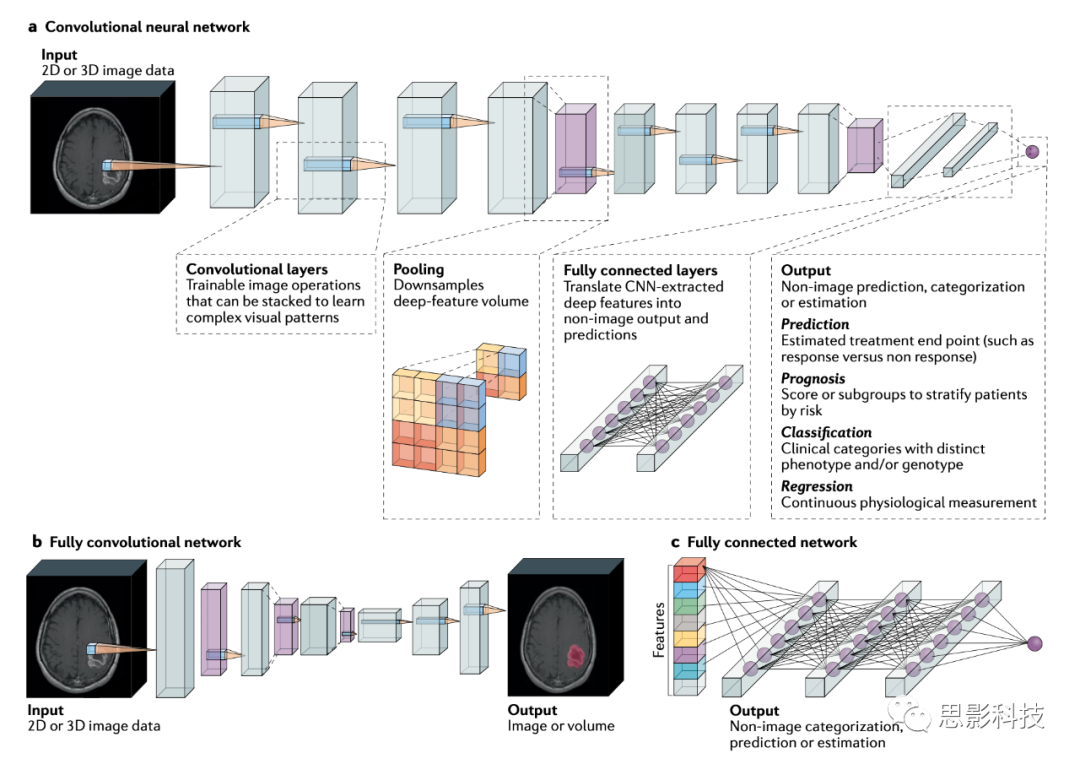
\includegraphics[width=\linewidth]{image/4/医疗影像与AI.png}
  \caption{常用于医学成像数据的神经网络的构造块和类型}
  \label{fig:my_label}
\end{figure}

通过应用影像组学和深度学习模型，个性化医疗能够识别出哪些患者最有可能从特定药物或治疗方法中受益，从而为每位患者量身定制最适合的治疗方案。这种方法不仅提高了治疗效果，延长了患者的生存期，还有效减少了不必要的副作用，提升了患者的生活质量。此外，AI技术的非侵入性特性使得医生能够在整个治疗过程中连续监测肿瘤的动态变化和微环境特征，及时调整治疗策略以应对疾病进展或治疗反应的变化。

此外，个性化医疗还通过整合多种数据源，包括影像数据、临床病理信息和基因组数据，提供全面的决策支持。这种多维度的数据融合不仅增强了预测模型的准确性，还揭示了肿瘤生物学的深层次机制，促进了放射基因组学的发展。最终，个性化医疗不仅为患者提供了更为精准和高效的治疗方案，也为临床医生提供了强大的工具，帮助他们在复杂的治疗环境中做出最优的医疗决策，从而全面改善癌症患者的预后和生活质量。

在心血管疾病管理方面，上海交通大学医学院附属瑞金医院引入了个性化医疗系统，利用AI分析患者的基因数据、生活方式和临床指标，制定个性化的预防和治疗方案。该系统能够预测患者患心血管疾病的风险，帮助医生制定个性化的健康管理计划，有效降低了疾病发生率。

此外，个性化医疗在遗传性疾病的筛查和治疗中也展现出巨大的潜力。例如，广东省的多家医疗机构启动了新生儿基因筛查项目，利用AI技术分析新生儿的基因数据，早期发现遗传性疾病的风险，从而及时采取干预措施，显著提高了治疗的成功率。

我国政府高度重视个性化医疗的发展，并出台了一系列政策以支持基因组学和人工智能(AI)技术在医疗领域的应用。国家卫生健康委员会发布了《生物医学新技术临床应用管理条例（征求意见稿）》，该条例明确了基因组数据的使用规范和隐私保护措施，为个性化医疗的发展提供了坚实的政策保障。此外，国家科技伦理委员会医学伦理分委员会也编制并发布了《人类基因组编辑研究伦理指引》，进一步规范了人类基因组编辑研究行为，促进了该领域研究的健康发展。

在地方层面，多个城市已经设立了个性化医疗试点项目。例如，深圳市双科医学研究院与招商仁和人寿保险有限公司签署了战略合作协议，共同推进“个性化医疗+创新保险”项目，开展“产-学-研-用”一体化转化研究与应用，实现深度融合建立重疾“防-控-保”解决方案，实施健康企业建设。这一合作不仅体现了政府与企业在个性化医疗领域的合作模式，也展示了通过科技创新推动健康中国建设的战略意图。通过这些政策和项目，我国在个性化医疗领域的发展正得到有力推动。

 \textbf{2.面临的挑战与未来展望}

尽管个性化医疗展现出巨大的潜力，但其发展仍面临诸多挑战。首先，基因组测序和分析的成本仍然较高，限制了个性化医疗的普及。随着技术的进步和规模效应的显现，测序成本有望逐步下降，使更多患者能够受益于个性化医疗服务。

其次，个人隐私和数据安全问题亟需解决。基因组数据的高度敏感性要求严格的隐私保护措施。为此，我国需要建立完善的数据管理和保护机制，确保患者的基因信息不被滥用。同时，相关法律法规的制定也至关重要，以规范基因组数据的使用，保护患者的隐私权和知情权。

此外，个性化医疗的推广需要跨学科的合作，包括基因组学、数据科学、临床医学等多个领域的协同发展。只有通过多方合作，才能充分发挥AI在个性化医疗中的优势，推动其在更多疾病领域的应用。

展望未来，随着基因组学和AI技术的不断进步，个性化医疗将更加精准和高效。AI将能够整合更多维度的数据，包括基因组、蛋白质组、代谢组等多组学数据，提供更加全面的健康评估和治疗方案。同时，个性化医疗将在慢性病管理、老年病治疗等领域发挥更大的作用，为人类健康带来更多福祉。

总的来说，个性化医疗作为智慧医疗的重要组成部分，正在通过基因组学和AI技术的深度融合，改变传统的医疗模式，提升医疗服务的精准度和有效性。随着技术的不断发展和政策的支持，个性化医疗将在未来的医疗体系中扮演越来越重要的角色，为人类健康保驾护航。

\subsection{智慧医院}

智慧医院是信息技术与医疗服务的完美结合，旨在通过人工智能（AI）、大数据分析和云计算等尖端技术优化医疗流程，提升医疗质量和效率。智慧医院不仅改善了医务人员的工作环境，还显著提升了患者的就医体验，同时优化了医院的管理流程。智慧医院主要涵盖三个方面：
第一，\textbf{面向医务人员的智慧医疗} 以电子病例为核心的信息化建设，方便医生查询和调阅病例信息，提高医疗服务的质量和效率。
第二，\textbf{面向患者的智慧服务} 包括智能导诊系统、智能排班系统和智能监控系统等，提供便捷的就医体验和高效的医疗服务。
第三，\textbf{面向医院管理的智慧管理} 涵盖财务结算、物资管理等多个方面，通过大数据分析和 AI 技术优化医院的资源配置和管理流程。

智慧医院建设解决了传统医院管理中信息孤岛、资源浪费和服务效率低下的问题，显著提升了医疗服务的效率和质量，增强了医院的核心竞争力。以下将详细探讨智慧医院的各个方面，并结合实际案例加以说明。

\begin{figure}[ht]
  \centering
  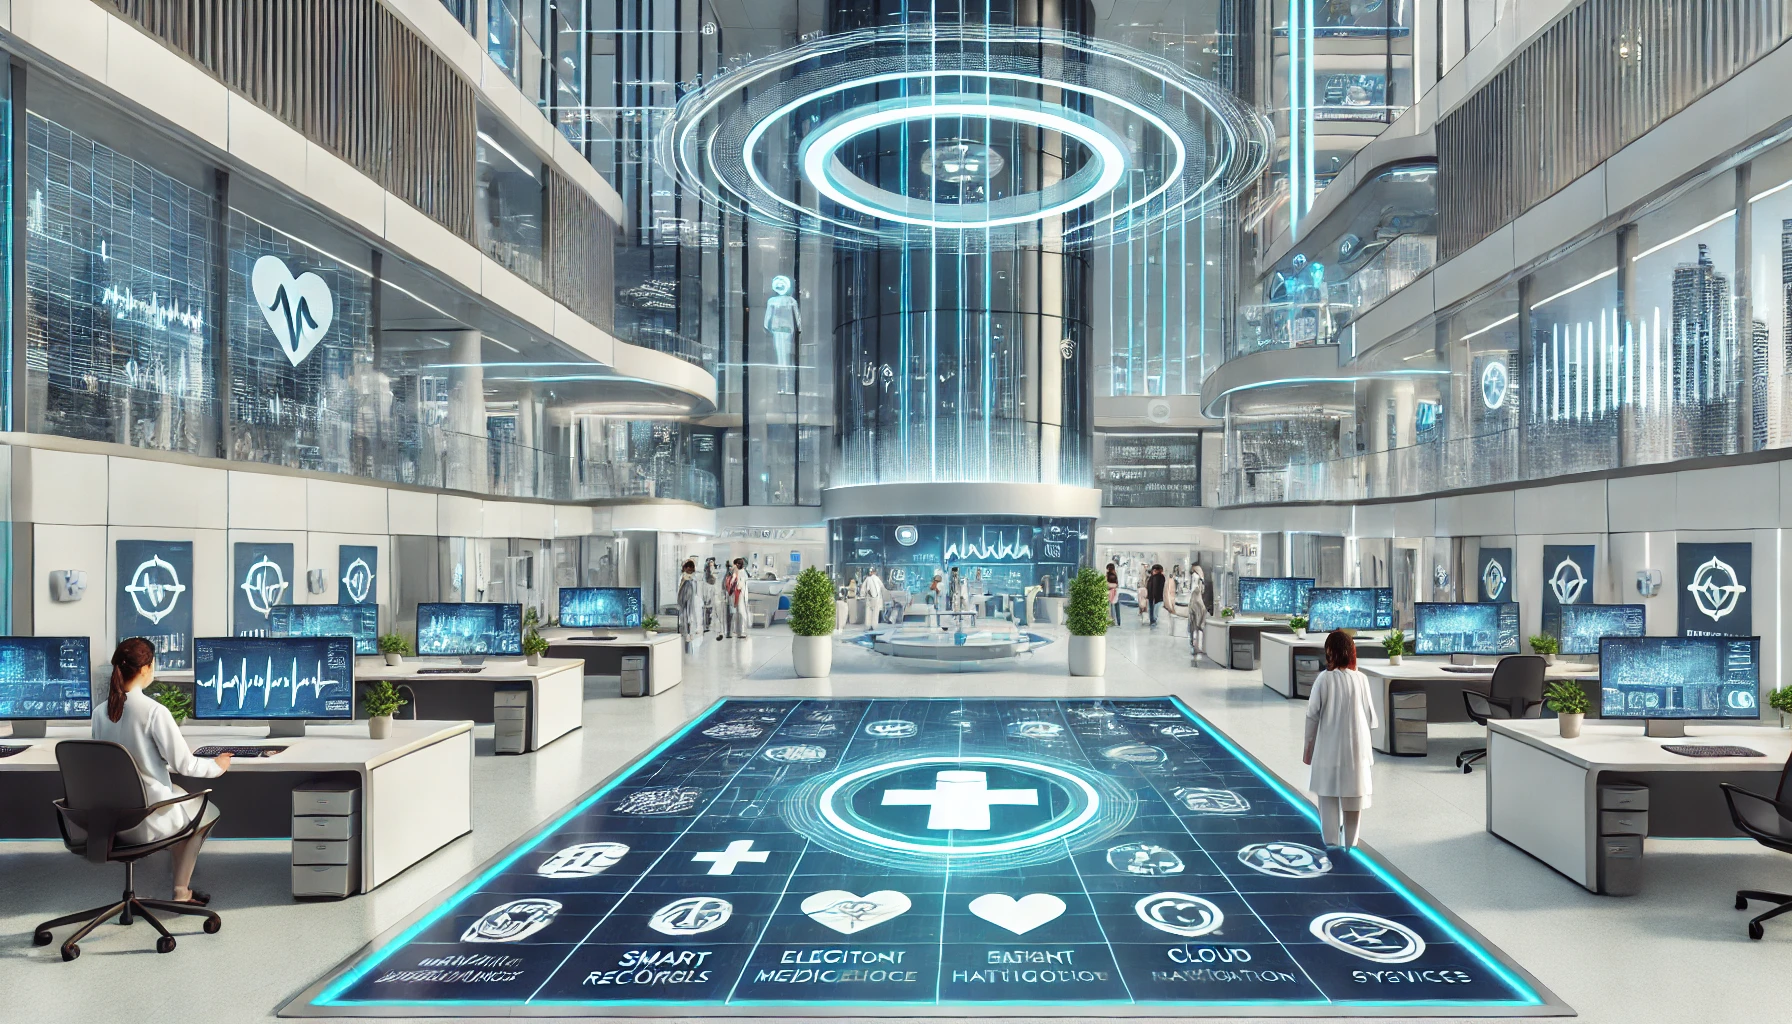
\includegraphics[width=\linewidth]{image/4/智慧医院.png}
  \caption{未来的智慧医院}
  \label{fig:my_label}
\end{figure}

\textbf{1.面向医务人员的智慧医疗}

智慧医疗系统以电子病例（Electronic Medical Records, EMR）为核心，通过信息化手段实现医务人员对患者信息的快速获取和管理。例如，阿里健康推出的“云医院”平台，通过整合患者的电子病历、检验结果和影像资料，医生可以在任何时间、任何地点访问患者的完整病历，提升了诊断的准确性和效率。

此外，智慧医疗还包括远程会诊和协作系统。北京协和医院与腾讯合作开发的远程医疗平台，利用AI技术支持多科室、多地区的专家进行远程会诊，实现了资源的优化配置和医疗服务的扩展。这不仅减轻了大医院的压力，也为偏远地区的患者提供了优质的医疗资源。

\textbf{2.面向患者的智慧服务}

智慧医院通过智能导诊系统、智能排班系统和智能监控系统等，提升了患者的就医体验。例如，杭州的某三甲医院引入了智能导诊机器人，患者可以通过语音或触屏与机器人互动，快速找到需要的科室和医生，减少了排队等候的时间。

智能排班系统利用AI算法，根据医生的专业特长、工作负荷和患者的需求，优化医生的排班安排，提高了医疗资源的利用效率。南京鼓楼医院实施的智能排班系统，有效减少了医生的轮班冲突，提升了整体医疗服务的协调性。

智能监控系统则通过实时监测患者的病情和医院的运营情况，确保医疗服务的连续性和安全性。例如，深圳某智慧医院部署了智能监控系统，能够实时监测重症监护室（ICU）患者的生命体征，并在出现异常情况时自动报警，及时干预，保障患者的安全。

\textbf{3.面向医院管理的智慧管理}

智慧管理涵盖财务结算、物资管理等多个方面，通过大数据分析和AI技术优化医院的资源配置和管理流程。以北京大学第一医院为例，他们引入了基于AI的库存管理系统，通过大数据分析预测药品和医疗器械的需求，优化库存水平，减少了资源浪费和库存积压。

在财务管理方面，智慧医院利用AI技术实现自动化结算和费用审核。上海华山医院采用的智能财务系统，能够自动识别和处理患者的医疗费用，减少了人工审核的错误率，提高了结算的速度和准确性。

此外，智慧医院还注重患者数据的整合与分析。通过构建统一的医疗数据平台，医院管理者可以实时获取医院的运营数据，进行全面的分析和决策支持。例如，广州市某智慧医院通过大数据分析优化了科室的运营流程，提升了整体医疗服务的效率和质量。

我国多个城市和地区已经展开了智慧医院的试点工作，取得了显著成效。例如作为中国智慧医疗的先行者，深圳市多家医院引入了AI辅助诊断系统、智能导诊机器人和远程医疗平台。深圳市政府还推动了“智慧医院示范工程”，通过政策支持和资金投入，促进智慧医疗技术的应用和普及。杭州通过与阿里健康的合作，建设了多个“云医院”，实现了医疗资源的线上共享和协同。智能导诊系统和智能排班系统的应用，大幅提升了患者的就医体验和医院的运营效率。北京协和医院与腾讯合作开发的远程会诊平台，为全国各地的患者提供了优质的医疗服务。同时，北京市政府推动智慧医疗基础设施建设，促进各大医院的信息化和智能化发展。

智慧医院的发展离不开技术的进步和政策的支持。我国政府高度重视智慧医疗的发展，出台了一系列政策文件，如《“健康中国2030”规划纲要》和《国家智慧医疗发展规划（2021-2025年）》，明确了智慧医疗的发展目标和路径。

在技术方面，5G技术的普及为远程医疗和实时数据传输提供了强有力的支持。华为和中兴等科技企业积极参与智慧医疗的建设，提供了先进的通信和计算基础设施，推动了智慧医院的快速发展。

\textbf{4.面临的挑战与未来展望}

尽管智慧医院在提升医疗服务质量和效率方面取得了显著成效，但其发展仍面临诸多挑战,如医疗数据的高度敏感性要求严格的隐私保护和安全保障。智慧医院需要建立完善的数据管理和保护机制，防止数据泄露和滥用。不同医院的信息系统和设备存在兼容性问题，缺乏统一的技术标准和接口，阻碍了智慧医疗技术的广泛应用和整合。智慧医院的建设需要大量的资金投入，尤其是在设备采购、系统开发和人员培训方面，如何降低成本、提高投资回报率是一个重要问题。智慧医疗的发展需要具备跨学科知识的专业人才，包括医疗、信息技术和数据科学等领域的人才，但目前相关人才的供给仍不足。

展望未来，随着技术的不断进步和政策的进一步支持，智慧医院将在以下几个方面取得更大的突破：1）AI技术将在医疗诊断、治疗方案制定和患者管理等方面发挥更大的作用，进一步提升医疗服务的精准度和个性化水平。2）物联网技术和可穿戴设备的普及，将实现患者的实时健康监测和数据采集，为智慧医疗提供更加全面和实时的数据支持。3）区块链技术将在医疗数据的存储和共享中发挥重要作用，确保数据的安全性和透明性，促进不同医疗机构之间的数据互联互通。4）虚拟现实（VR）和增强现实（AR）技术将在医学教育、手术培训和患者康复等方面得到广泛应用，提升医疗服务的多样性和互动性。

总的来说，智慧医院作为智慧医疗的重要组成部分，正在通过信息技术与医疗服务的深度融合，改变传统的医疗模式，提升医疗服务的质量和效率。随着技术的不断进步和政策的持续支持，智慧医院将在未来的医疗体系中发挥越来越重要的作用，为人类健康保驾护航。

\subsection{医学影像与医疗诊断辅助}
医学影像诊断与医疗诊断是人工智能（AI）在医疗领域应用最为广泛和关键的两个方面。随着深度学习算法和大数据分析技术的不断进步，AI不仅能够快速、准确地分析大量医学影像数据，还能在整体医疗诊断过程中提供智能化支持，帮助医生制定个性化的治疗方案，极大地提升了医疗服务的效率和质量。

\begin{figure}[ht]
  \centering
  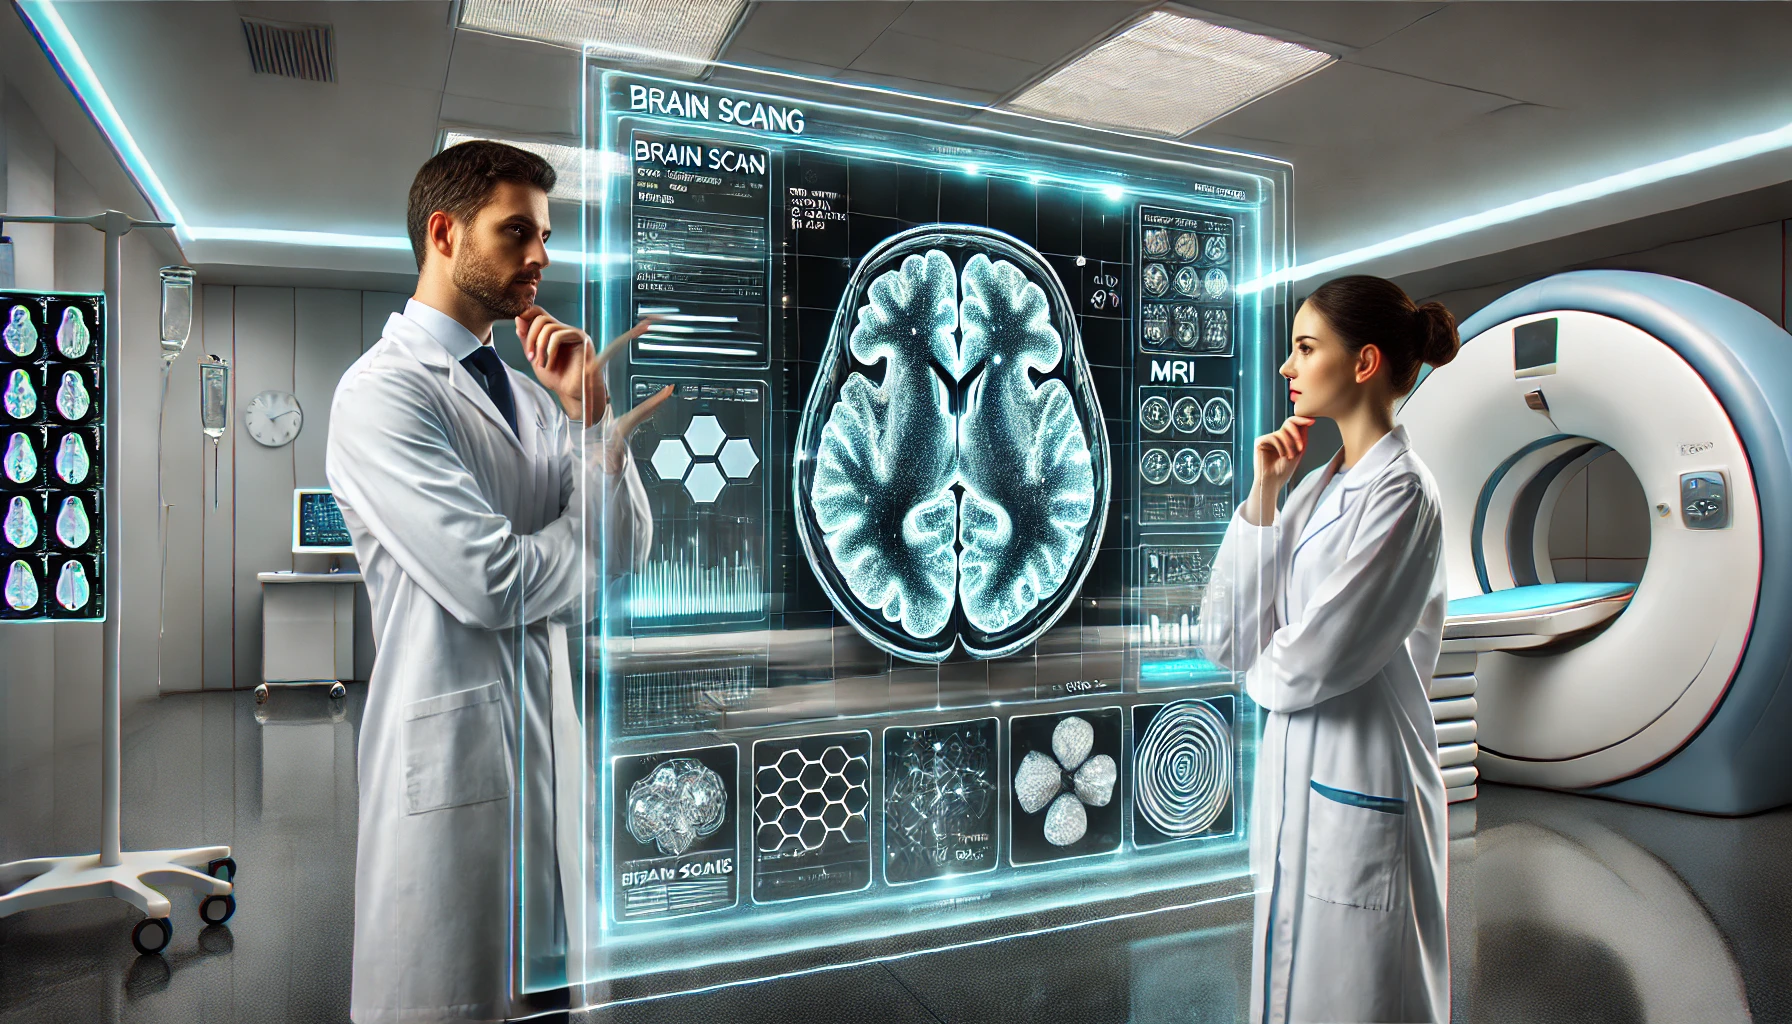
\includegraphics[width=\linewidth]{image/4/医疗影像处理.png}
  \caption{AI辅助医疗影像处理}
  \label{fig:my_label}
\end{figure}

在医学影像诊断方面，AI技术通过深度学习算法能够自动识别和分析医学影像中的异常情况。例如，百度的“飞桨”深度学习平台已经应用于肺部CT扫描中的肿瘤检测，通过训练深度学习模型，AI能够准确识别肺部结节的位置、大小及其恶性程度，辅助医生进行早期癌症筛查和诊断。阿里健康与浙江大学医学院合作开发的智慧影像系统，能够将CT、MRI和超声影像数据进行整合分析，提供综合性的诊断报告，帮助医生更全面地了解患者的病情。此外，华为与北京大学第一医院合作开发的智能手术导航系统，利用AI技术实时监测手术区域的影像，指导医生进行微创手术，提高手术的成功率和安全性。

在医疗诊断领域，AI被誉为“魔法助手”，通过分析大量的临床数据，帮助医生发现潜在的健康问题，制定个性化的治疗方案。例如，腾讯医疗联合清华大学开发的智能诊断系统，利用机器学习算法分析心电图数据，能够准确预测心脏疾病的风险，帮助医生制定预防和治疗计划。阿里健康的智能药物推荐系统，通过分析患者的基因信息和病历数据，为癌症患者推荐最适合的靶向药物和治疗方案，显著提高了治疗效果，减少了副作用。同时，京东健康推出的智能健康管理平台，利用AI算法监控糖尿病患者的血糖数据和饮食习惯，实时提供健康建议，帮助患者有效控制病情。

实际应用中，北京协和医院与腾讯合作开发的远程诊断平台，利用AI技术进行病例分析和疾病预测，能够快速处理海量的医疗数据，辅助医生进行远程会诊，提高了诊断的效率和准确性，特别是在急诊和重症监护中发挥了重要作用。上海交通大学医学院附属瑞金医院引入的基于AI的智能诊断系统，通过分析患者的基因组数据和临床指标，制定个性化的预防和治疗方案，在心血管疾病和遗传性疾病的管理中取得了显著成效，降低了疾病发生率，提升了患者的生活质量。广东省多家医疗机构启动的新生儿基因筛查项目，利用AI技术分析新生儿的基因数据，早期发现遗传性疾病的风险，实现了早期干预和治疗，显著提高了遗传性疾病的治愈率。

我国政府高度重视AI在医学影像诊断和医疗诊断中的应用，出台了一系列政策文件支持相关技术的发展。例如，《国家智慧医疗发展规划（2021-2025年）》明确提出要推动AI技术在医疗诊断中的应用，提升医疗服务的智能化水平。同时，国家卫生健康委员会也发布了相关指导意见，规范AI在医疗领域的应用，确保其安全、有效和可持续发展。在技术支持方面，华为、阿里健康、腾讯等科技企业积极参与智慧医疗建设，提供先进的AI算法和数据分析平台，推动医疗机构的信息化和智能化发展。例如，华为的“云医”平台通过AI技术支持医学影像分析和疾病预测，助力全国各地的医疗机构提升诊断水平。

尽管AI在医学影像诊断和医疗诊断中展现出巨大的潜力，但其发展仍面临诸多挑战。首先，医疗数据的高度敏感性要求严格的隐私保护和安全保障，智慧医疗需要建立完善的数据管理和保护机制，防止数据泄露和滥用。其次，AI算法需要在多样化的临床环境中进行验证，确保其诊断和预测的准确性，避免误诊和漏诊。此外，不同医疗机构的信息系统和设备存在兼容性问题，缺乏统一的技术标准和接口，阻碍了AI技术的广泛应用和整合。同时，AI技术的研发和应用成本较高，限制了其在中小型医疗机构中的普及，随着技术的进步和规模效应的显现，AI技术的成本有望逐步下降，使更多医疗机构能够负担并应用AI技术。此外，智慧医疗的发展还需要具备跨学科知识的专业人才，包括医疗、信息技术和数据科学等领域的人才，但目前相关人才的供给仍不足。

展望未来，随着AI技术的不断进步和完善，其在医学影像诊断和医疗诊断中的应用将更加广泛和深入。基于大数据和深度学习的AI算法将能够整合更多维度的数据，包括基因组、蛋白质组和代谢组等多组学数据，提供更加全面和精准的健康评估和治疗方案。同时，AI技术将在慢性病管理、老年病治疗等领域发挥更大的作用，提升整体医疗服务的水平。区块链技术将在医疗数据的存储和共享中发挥重要作用，确保数据的安全性和透明性，促进不同医疗机构之间的数据互联互通。虚拟现实（VR）和增强现实（AR）技术将在医学教育、手术培训和患者康复等方面得到广泛应用，提升医疗服务的多样性和互动性。

\begin{figure}[ht]
  \centering
  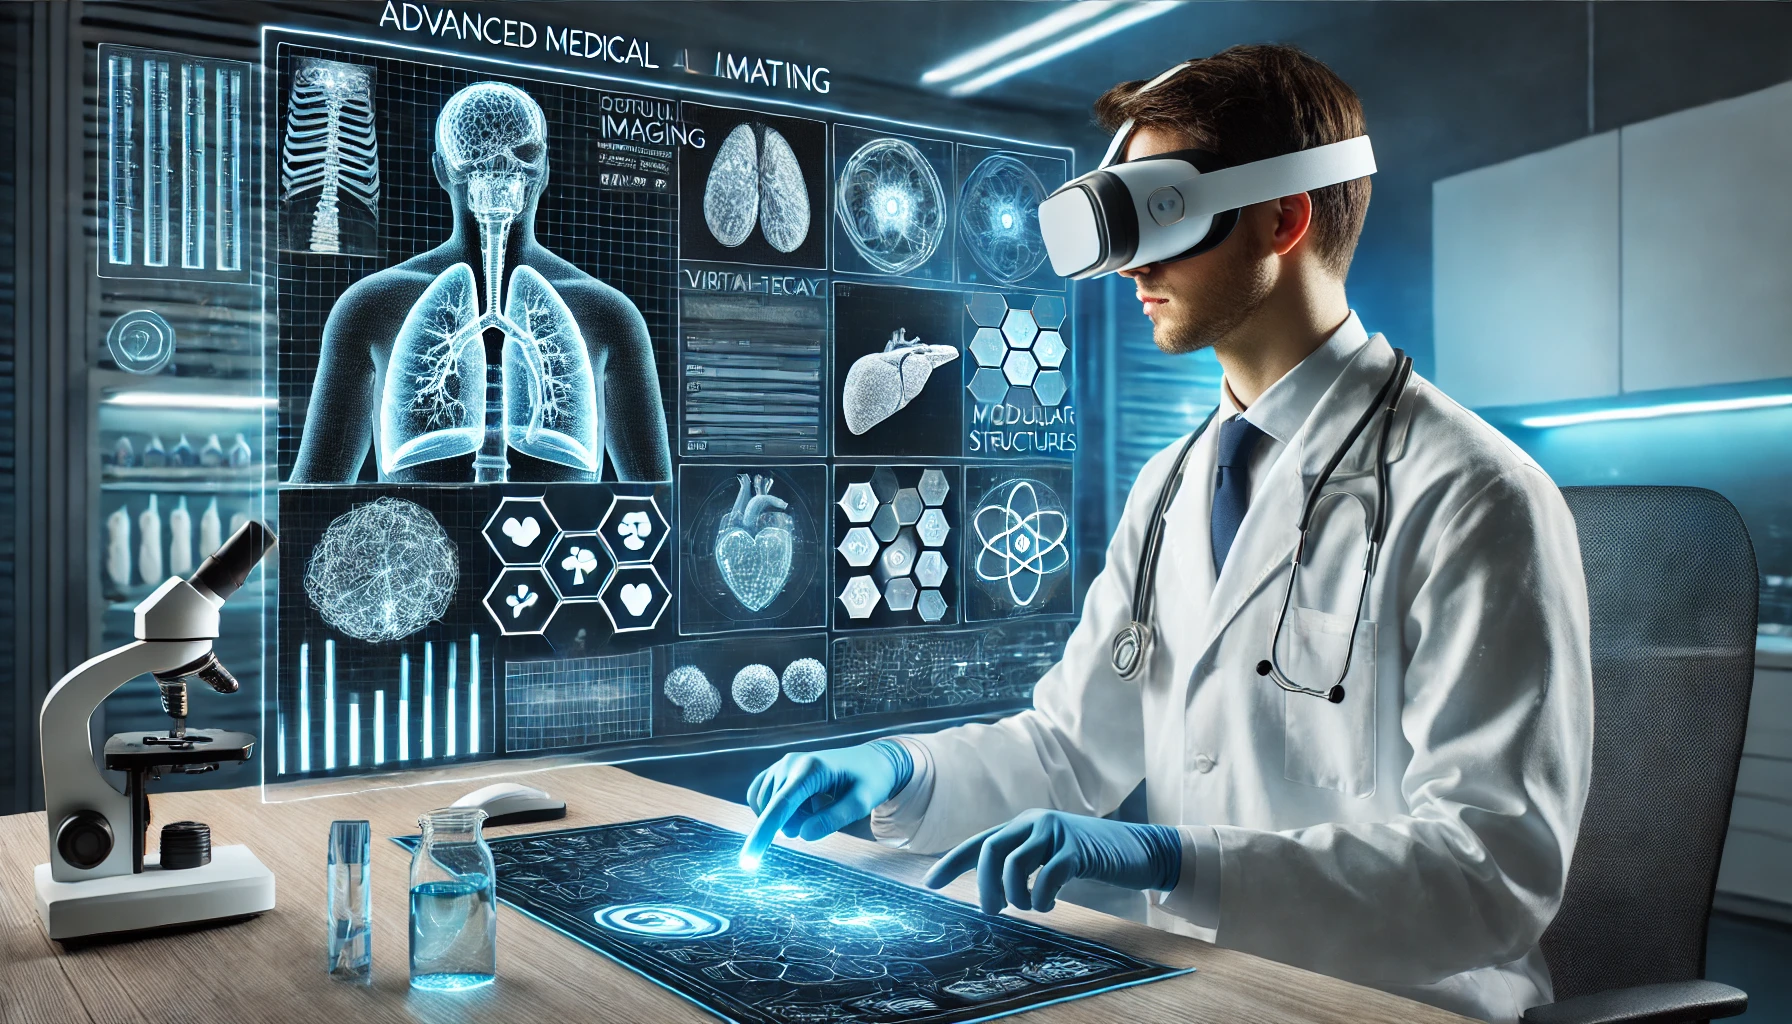
\includegraphics[width=\linewidth]{image/4/VR诊断.png}
  \caption{未来使用VR技术对患者进行远程诊断}
  \label{fig:my_label}
\end{figure}

总的来说，医学影像诊断与医疗诊断是AI在智慧医疗中应用的重要领域。通过深度学习算法和大数据分析，AI不仅提高了诊断的准确性和效率，还为医生提供了智能化的决策支持，促进了个性化医疗的发展。尽管面临数据隐私、安全性和技术整合等挑战，随着技术的不断进步和政策的支持，AI将在医学影像诊断和医疗诊断中发挥越来越重要的作用，推动智慧医疗的发展，为人类健康保驾护航。

\subsection{挑战与未来发展}
尽管AI在智慧医疗中展现出巨大的潜力，但其发展仍面临诸多挑战。医疗数据的敏感性要求高度的隐私保护和安全保障，必须建立完善的数据管理和保护机制。AI算法需要在多样化的临床环境中进行验证，确保其诊断和预测的准确性，避免误诊和漏诊。智慧医疗的应用涉及复杂的法律和伦理问题，需要制定相应的法规，确保AI技术的合理和负责任的使用。尽管AI技术逐渐成熟，但其高昂的研发和应用成本仍限制了其在全球范围内的普及，需要进一步降低成本，提升技术的可及性。

展望未来，随着AI技术的不断进步和完善，其在智慧医疗中的应用将更加广泛和深入。基因组学和生物技术的结合，将推动精准医学的发展；AI在医疗机构管理中的应用，将进一步提升医疗服务的效率和质量；远程医疗和虚拟护理助手的普及，将使医疗服务更加普惠和便捷。智慧医疗的持续发展，将为人类健康和福祉带来更多的福祉，推动全球医疗行业的数字化转型和升级。

智慧医疗是AI技术在医疗领域的重要应用，涵盖了个性化医疗、智慧医院、医学影像诊断辅助、医疗诊断及其他多方面的应用。通过优化医疗流程、提升诊断准确性和效率、提供个性化治疗方案，AI正在深刻改变传统医疗模式。然而，智慧医疗的发展也面临数据隐私、算法可靠性和成本等挑战。未来，随着技术的不断进步和相关机制的完善，智慧医疗将为人类健康带来更加美好的未来。

\newpage
\section{智慧农业}

智慧农业是现代农业的一种发展趋势，指的是利用先进的信息技术、人工智能、大数据、物联网（IoT）、机器人技术等手段，通过对农业生产、管理和决策的数字化、智能化升级，实现更高效、精准、可持续的农业生产方式。随着全球人口的不断增加和农业资源的紧张，传统农业模式已经难以满足未来对粮食、安全、环保等多方面的需求。在此背景下，智慧农业作为提升农业生产效率、确保粮食安全和实现可持续发展的关键方案，受到了全球范围的广泛关注。

智慧农业的核心在于精准农业、数据驱动的决策支持系统以及对资源的最优配置。通过传感器、卫星遥感、无人机等设备获取实时数据，结合人工智能的分析和预测能力，智慧农业不仅可以提高作物的产量和质量，还能够优化农业资源的利用，减少环境污染，并增强农业的应对气候变化能力。

本节将深入探讨智慧农业的三个重要方面：首先，介绍\textbf{什么是智慧农业}，理解其基本概念和技术架构；接着，探讨\textbf{农业生产中的智能化应用}，分析其在作物种植、农业管理和资源利用方面的具体实现方式；最后，展望\textbf{智慧农业的未来发展与挑战}，讨论其在全球范围内的应用潜力以及发展中面临的技术、环境和社会挑战。



通过本节内容，读者将对智慧农业的概念、应用技术和未来前景有一个全面深入的了解，理解人工智能和先进技术如何在现代农业中发挥关键作用，推动农业生产方式的转型升级。

\subsection{什么是智慧农业}

\begin{figure}[ht]
  \centering
  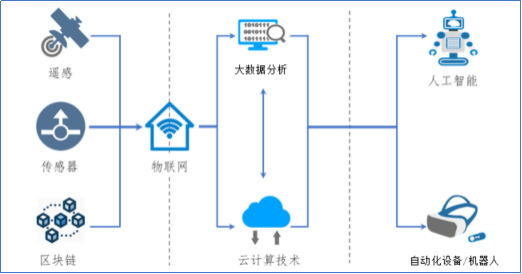
\includegraphics[width=0.8\linewidth]{image/4/4_4智慧农业核心组成.png}
  \caption{智慧农业核心组成（待优化）}
  \label{fig:my_label}
\end{figure}

智慧农业是现代农业的一个重要发展方向，代表着农业生产管理从传统手工操作、
经验积累向基于信息技术、数据分析和智能化技术的现代化转型。它通过集成先进的技
术，如物联网（IoT）、人工智能（AI）、大数据、云计算技术、自动化设备等，使农业生产
更加精准、高效、可持续。

智慧农业的核心是通过对农业生产全过程（如土壤质量监控、作物生长监测、病虫
害预测、水资源管理等）的实时监控与数据分析，从而实现更智能的决策支持和资源配
置。与传统农业相比，智慧农业能够减少对人工和资源的依赖，同时最大化产出，提高
作物质量，并减少环境负担。

\subsubsection{1. 智慧农业的基本概念}

智慧农业是一种以高新技术为支撑的现代农业模式，如图4.9所示智慧农业通过物联网（IoT）、人工智能（AI）、大数据分析与云计算技术和自动化设备与机器人等先进技术，全面提升农业生产的智能化水平。以下分别从这些技术的应用角度详细说明智慧农业的内涵。
\begin{enumerate}[(1)] 
  \item \textbf{物联网（IoT）}
  
    物联网技术是智慧农业的基础，其核心在于利用传感器、无线通信技术和数据采集设备，实现农业生产环境和作物生长状态的实时监测与动态反馈。通过分布式传感器网络，可以获取诸如土壤湿度、空气温湿度、光照强度、二氧化碳浓度、风速风向等关键农业参数。这些数据通过无线传输技术（如Wi-Fi、LoRa或5G）被实时汇总到云端管理系统，供农业管理者通过可视化平台随时查看并进行深度分析，从而支持科学决策。
    
    例如，智能灌溉系统利用传感器采集的土壤湿度和气象数据，可以精准控制灌溉的时间、频率和水量，不仅大幅度节约了水资源，还为作物提供了适宜的生长环境，提升了农产品的质量和产量。除此之外，物联网技术还可以应用于温室监控、病虫害预警、牲畜定位与健康监测等场景。例如，在温室大棚中，传感器实时感知温度和湿度变化，系统可以自动调节通风设备或喷淋系统，保持适宜的作物生长条件。
    
    通过物联网的深度应用，农业生产从被动管理转变为主动监测与精准控制，实现了全流程的数字化和智能化。这不仅降低了劳动强度和资源浪费，还为农业管理者提供了更加高效和经济的生产模式，推动了农业的现代化转型。

  \item \textbf{人工智能（AI）}
  
    人工智能技术在智慧农业中发挥着重要作用，主要用于数据分析、趋势预测和智能决策支持。通过先进的机器学习和深度学习算法，AI可以从海量农业数据中提取有价值的信息，识别作物生长模式、预测病虫害发生，并提供针对性的防治方案。例如，基于AI驱动的图像识别技术，农业管理者可以分析作物叶片的健康状况，精准判断是否存在病害，并快速制定应对措施。这种智能检测方式不仅提高了病虫害管理的效率，还减少了过度使用农药的风险，保护了生态环境。
    
    此外，人工智能还在农业机器人控制中得到广泛应用，使机器人能够胜任复杂且高精度的任务。例如，AI支持的机器人可以完成精准播种，根据土壤条件和作物生长需求控制种子间距和深度；在除草方面，机器人能够识别杂草并通过机械方式或定向喷洒除草剂进行清理，从而减少化学药剂的使用；在施肥方面，AI可基于土壤和作物状态，指导机器人实现分区精准施肥，既提高肥料利用率，又避免因过量施肥造成的土壤污染。
    
    更进一步地，人工智能还可以结合无人机、传感器网络和物联网平台，为大规模农业生产提供端到端的智能化支持。例如，无人机搭载AI视觉系统，可以高空监测作物生长状况，并生成全田地的健康评估报告，为农场管理提供数据支撑。
    人工智能的智能预测和决策能力，不仅显著提高了农业生产效率，还大幅减少了资源浪费，使农业生产更加环保和可持续化。通过AI技术的深入应用，智慧农业正在实现从经验驱动向数据和算法驱动的根本转变，为现代农业发展注入了强大的技术动力。

  \item \textbf{大数据分析与云计算技术}
  
    大数据分析与云计算技术是智慧农业的核心支柱，两者协同作用，为农业生产提供科学的决策支持和深度洞察，推动农业向精细化、智能化方向迈进。
    
    大数据分析通过整合和处理来自多种渠道的大量数据，如传感器网络、无人机、卫星遥感和气象观测站，帮助农业管理者实现全面的环境感知和精准的决策支持。例如，大数据技术能够整合土壤湿度、气象变化、作物生长状态等信息，生成土地肥力分布图，揭示作物生长规律，并分析市场需求趋势。这些洞察为优化生产计划、制定精准种植策略和规避气候风险提供了可靠依据。
    
    具体而言，通过对历史气象数据和作物产量数据的分析，可以构建农作物产量预测模型，帮助预测未来的产量水平，指导种植者调整作物种植结构以适应市场需求。此外，大数据分析还可以用于提前识别病虫害风险，通过早期预警机制帮助农业管理者制定科学的防治方案。这不仅减少了农药的使用，降低了环境负担，还显著提高了作物的品质和经济价值。
    云计算技术为大数据分析提供了强有力的支撑，尤其是在数据存储和高效计算方面表现出色。通过云计算，海量农业数据可以快速进行实时处理，同时为复杂算法模型的构建提供弹性的计算资源。云计算的集中化存储和分布式计算能力，不仅显著降低了农业企业的基础设施建设成本，还使农业管理系统具有更强的扩展性和灵活性。例如，当传感器网络收集到大量实时数据时，云平台可以动态分配计算资源，迅速完成数据分析，并将结果通过可视化界面展示给农业管理者，用于即时决策支持。
    
    更重要的是，云计算技术还推动了农业服务模式的创新。例如，基于云计算的农业平台可以提供远程作物监控、智能灌溉管理、病虫害诊断等服务，帮助农业从业者轻松应对复杂的生产管理任务。云计算还能够支持不同农业生态系统的数据共享和协同，为跨区域农业合作和大规模农业项目提供技术保障。
\item \textbf{自动化设备与机器人} 

    自动化设备和机器人已成为智慧农业的重要执行工具，为农业生产带来了革命性的变化。现代农业机械，如自动驾驶拖拉机、精准播种机和无人植保机，能够大幅提高农业操作的效率和精准度，减少人工干预的同时降低生产成本。自动驾驶拖拉机通过先进的导航和控制技术，能够自动完成耕作、播种等多种任务，精准度远超人工操作；精准播种机通过精确计算播种深度和密度，确保每一粒种子都能在最佳位置发芽生长；无人植保机则能够对农田进行高效的植保作业，通过自动飞行、精准喷洒农药，实现了作物保护的精准施用，减少了药剂的浪费和环境污染。 农业机器人更是进一步推动了农业作业的自动化，能够完成一些更为复杂的任务。

    例如，果实采摘机器人通过AI算法和视觉识别技术，能够判断果实的成熟度，并根据不同的果实类型、位置和周围环境，选择最优的采摘路径，精准地进行采摘。这不仅大大提高了采摘效率，还能减少人为操作对果实的损伤。 此外，温室管理系统中的自动化设备也发挥着至关重要的作用。通过集成的温控、湿控和光照控制系统，这些设备能够根据实时监测的数据，自动调节温度、湿度和光照，为作物提供最佳的生长环境。这一系列自动化设备和技术的普及，使得农业生产从过去以大量人力为基础的劳动密集型模式，逐渐转变为以技术为驱动的智能化、精细化生产模式，不仅提升了农业的生产效率，还增强了农产品的质量和市场竞争力，推动了农业的可持续发展。
\end{enumerate} 

综上所述，物联网、人工智能、大数据分析与云计算技术，以及自动化设备和机器人，构成了智慧农业的核心支撑，推动了农业生产的数字化、智能化和精细化发展。通过实时监测、精准控制、数据分析和智能决策，这些技术不仅显著提高了生产效率，降低了资源浪费，还提升了农产品的质量和市场竞争力。随着这些技术的不断融合与应用，智慧农业正逐步实现从传统劳动密集型向技术驱动型转变，推动着农业向可持续、环保和高效的方向发展，为全球农业生产的未来注入了强大的技术动力。 




\subsubsection{2. 智能农业的组成部分}

智慧农业作为现代农业技术发展的前沿领域，其核心在于充分利用物联网、大数据、云计算等先进信息技术，实现农业生产的高效化、环保化和可持续发展。如图 XXX 所示，这一目标的实现依赖于四大关键环节：数据采集、数据传输与存储、数据分析与决策支持，以及执行与自动化。以下内容将围绕这四个部分进行阐述：
\begin{figure}[ht]
  \centering
  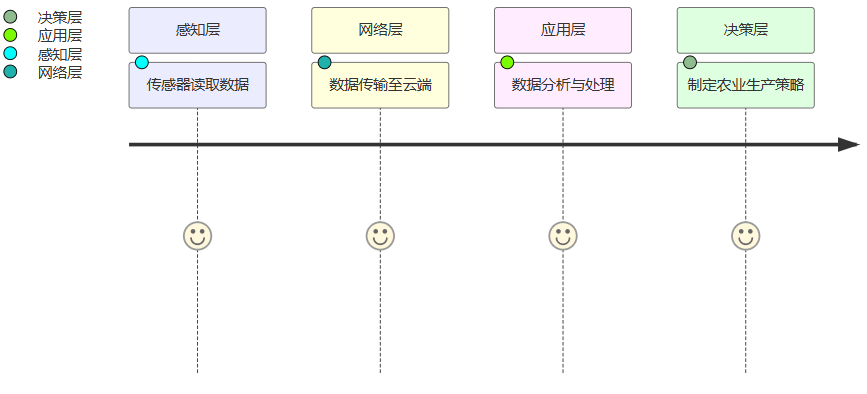
\includegraphics[width=0.8\linewidth]{image/4/4_4智慧农业的组成部分.png}
  \caption{智慧农业组成部分（待优化）}
  \label{fig:my_label}
\end{figure}
\begin{enumerate} % 设置列表编号为带括号的形式
  \item 数据采集
  
    智慧农业的第一步是通过传感器、无人机和遥感技术等设备对农业环境和作物生长状态进行数据采集。传感器网络分布在农田、温室或养殖场内，实时监测诸如土壤湿度、空气温湿度、光照强度、二氧化碳浓度、病虫害情况等关键参数。此外，无人机和卫星遥感还可以提供大范围的作物生长影像和农田全景数据。高质量的数据采集是后续分析和决策的基础。

  \item 数据传输与存储
  
    采集到的数据需要通过无线传输技术（如Wi-Fi、LoRa或5G）实时传送至云端或本地数据中心进行存储。云计算技术在这一环节发挥关键作用，确保海量数据的高效存储和分布式处理能力。此外，边缘计算设备可以对部分数据进行本地预处理，减少传输延迟，提升系统实时性。这一环节为数据分析与决策提供了充足的支持。

  \item 数据分析与决策支持
  
    在数据传输和存储后，通过大数据分析和人工智能技术对数据进行处理和挖掘，提取有价值的信息。例如，大数据分析可以揭示作物生长模式、预测病虫害风险，人工智能算法则可以基于历史数据和实时信息生成精准的种植、灌溉和施肥方案。决策支持系统通过可视化平台向农业管理者提供清晰的建议或自动生成优化方案，帮助他们做出科学决策。

  \item 执行与自动化
  
    基于分析和决策的结果，通过自动化设备和机器人执行具体操作。例如，智能灌溉系统根据土壤湿度数据精准调控水量；农业机器人根据AI指令进行果实采摘或除草；无人机根据作物健康评估图进行精准喷洒农药。这一环节实现了决策的快速落地，将智能化转化为实际生产力。
\end{enumerate}

\subsubsection{3. 智慧农业的优势与潜力}


智慧农业以其显著的优势，在现代农业中展现出广阔的发展潜力。首先，智慧农业通过自动化设备与智能管理，大幅提升了生产效率。例如，无人驾驶农机和智能灌溉系统的应用，使农事操作更加精准高效，同时有效减少了人力投入与操作误差。此外，智慧农业充分利用物联网与大数据技术，根据作物的实际需求优化水肥管理，从而显著降低资源浪费，减少生产成本。

在农产品质量与安全性方面，智慧农业通过全程溯源管理，借助区块链和传感技术，确保从田间到餐桌的每一个环节都透明可追溯。这不仅提升了消费者对农产品质量的信任，也推动了农业品牌化发展。同时，智慧农业在环境保护方面表现出色。精准施肥与合理用药等技术的应用，不仅有效降低了化学品的过度使用，还减少了农业生产对生态环境的负面影响，推动了绿色与可持续发展。

智慧农业的潜力同样令人瞩目。首先，它显著增强了农业生产的抗风险能力。通过遥感技术和大数据分析，农业生产者能够提前预测极端天气、病虫害等潜在风险，保障生产的稳定性。其次，智慧农业为精准农业的实现提供了坚实基础，将传统粗放式管理模式转变为单株或单亩级的精细化管理，大幅提高了生产效率与产量。此外，智慧农业加速了农业的数字化转型，综合运用物联网、云计算和人工智能技术，推动了农业现代化进程。

智慧农业还为农业与其他产业的融合提供了新契机，例如生态旅游与农业科普等新兴业态的快速发展，为农村经济注入了活力。在全球化背景下，智慧农业能够有效应对粮食安全的压力。通过提高生产效率和优化供应链管理，它保障了全球粮食供给的稳定性。同时，智慧农业也成为前沿科技的实践沃土，推动物联网、人工智能与区块链等技术的不断创新与应用。

综上所述，智慧农业以其卓越的优势和巨大的发展潜力，既能有效应对当前农业面临的诸多挑战，又为未来农业的可持续发展提供了创新解决方案和战略路径。


\subsection{农业生产中的智能化应用}

随着科技的不断进步，智慧农业正在逐渐改变传统的农业生产模式。智能化应用通过人工智能、大数据、物联网（IoT）、无人机、机器人等先进技术，使农业生产过程更加精细化、高效化，并减少资源浪费，提升产量和质量。这些技术不仅能优化农田管理，还能大幅提高农业的可持续性，推动农业现代化进程。

本节将详细探讨农业生产中的智能化应用，涵盖智能灌溉、无人机和机器人在农田管理中的应用等方面，展示如何通过科技手段实现农业生产的智能化管理。

\subsubsection{1. 智能灌溉系统}

智能灌溉系统是一种基于先进技术的现代农业灌溉解决方案，旨在优化水资源利用，提高农业生产效率。灌溉作为农业生产中的基础环节，传统方法通常依赖人工判断天气和土壤湿度，可能导致水资源浪费或灌溉不足。而智能灌溉系统通过集成传感器、物联网和大数据分析技术，实现对环境和作物需求的精确感知和管理。

具体来说，系统通过传感器实时监测土壤湿度、天气预报和作物生长状态等数据，利用物联网技术将信息传递到中央控制单元，并通过大数据分析计算最优灌溉方案。根据分析结果，系统能够自动调整灌溉量，确保作物获得所需水分，避免浪费水资源或供水不足。

\textbf{1.1 智能灌溉的工作原理} \\
智能灌溉系统通过多层次的架构设计，集成多种先进技术，实现了精准、高效的灌溉管理。该系统的运行基于对环境和作物数据的全面感知与智能分析，涵盖从数据采集到执行控制的完整流程。如图xxxxx，所示其工作原理可以划分为以下五个主要层次：

\begin{figure}[ht]
  \centering
  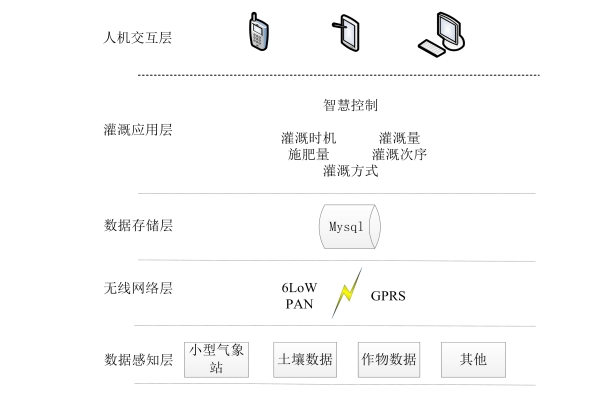
\includegraphics[width=0.8\linewidth]{image/4/4_4智能灌溉.png}
  \caption{智能灌溉系统架构图（待优化）}
  \label{fig:my_label}
\end{figure}

\textbf{数据感知层}是整个系统的基础，通过各种传感器实时采集与灌溉相关的环境数据。这些数据包括小型气象站提供的温湿度、降雨量等气候信息，土壤传感器监测的土壤湿度与养分含量，作物生长传感器获取的植物状况，以及其他环境数据。这些传感器通过分布式布局，实现了对农田状况的全面感知。

无线网络层负责将采集到的数据传输到中央数据存储或处理单元，常用的通信技术包括6LoWPAN和GPRS等，前者适用于短距离、低功耗的数据传输，后者则适用于广域范围的数据通信。无线网络的应用确保了数据传输的实时性和稳定性，为系统的高效运行提供了有力支持。


\textbf{数据存储层}通过数据库（如MySQL）对传输来的环境与作物数据进行集中存储和管理。数据库的设计确保了数据的安全性与高效性，并为后续的数据分析与应用提供了支撑。


\textbf{灌溉应用层}是系统的核心功能模块，通过智能控制算法对灌溉进行精准管理。根据存储的环境数据与作物需求，该层可以动态调整灌溉时机、灌溉量、施肥量、灌溉顺序以及灌溉方式。基于智能分析的决策过程，显著提高了水资源利用效率，并保证了作物的健康生长。

\textbf{人机交互层}为用户提供了便捷的系统操作与管理界面。用户可以通过智能手机、平板电脑或计算机监控灌溉状况，并对系统设置进行调整。这一层实现了系统的可视化与远程操作，使管理过程更加直观和高效。

通过数据感知、无线通信、数据存储、智能控制和人机交互五个层次的协调运作，智能灌溉系统实现了精准、高效、智能化的农业灌溉管理。这一系统不仅提升了农业生产效率，优化了资源利用，还为农业现代化提供了坚实的技术支撑，推动了可持续农业的发展。

\textbf{1.2 智能灌溉应用实例} \\
智能灌溉系统在不同的农业环境和需求中已经取得了显著的应用成果，以下是几个典型实例：

苏美仑智慧农业在温州科技园教研实训基地实施的智能水肥一体化项目，主要目的是提升农业灌溉系统的智能化管理水平。该项目通过使用水肥一体机，实现了以下几方面的应用效果：首先，智能化水肥供给功能使得水肥一体机能够根据季节变化、土壤水分状况、作物类型和肥料需求，自动调节水肥比例，确保作物获得适量的水分和营养。其次，精确灌溉与施肥技术使得设备能够通过精确控制施肥量和时间，将肥料溶液均匀施于作物根部，这不仅提升了农作物的产量和品质，还减少了环境污染。再次，实时监控与预警系统具备实时监控功能，能够监测灌溉系统的运行状态，及时发现并预警异常情况，如水源不足、系统泄漏等，确保灌溉系统的高效运行。此外，自动阀门控制功能通过监测土壤湿度、气候条件和作物生长情况，系统可以自动控制阀门的开关，提高灌溉效率，节约水资源。苏美仑水肥一体机在温州科技园的应用显著提升了农业生产效率，实现了对作物生长环境的精准控制，有助于提高农产品的产量和质量，同时也为环境保护作出了贡献。

湖南省桃江县大田智慧农业项目是一个集环境监测、土壤墒情监测、智能虫情监测和智能灌溉于一体的现代化农业管理项目，通过安装小型自动气象站、土壤墒情监测站、智能虫情测报站和智能灌溉控制器等设备，实现了对农田环境的实时监测、病虫害的智能预警以及根据土壤状况自动调节灌溉，通过智慧农业管理平台对各类数据进行集中展示和分析，从而提高了农业生产的智能化、自动化水平，有效提升了作物产量和品质，推动了农业资源的合理利用和可持续发展。
\subsubsection{2. 精准施肥与智能农药喷洒}

精准施肥与智能农药喷洒是智慧农业的重要组成部分，旨在通过科技手段实现作物生长所需养分的精准供给，以及病虫害防治的精确投放。这不仅可以提高作物的产量和质量，还能避免肥料和农药的过度使用，减少对环境的污染。



\subsubsection{3. 无人机与机器人在农业中的应用}

无人机和机器人技术是推动智慧农业发展的关键技术，特别是在大规模农业生产中，能够显著提高农业生产的自动化水平，减少人工成本，增加作物的产量和质量。

\textbf{2.1 无人机在农业中的应用} \\
农用无人机作为现代农业技术的重要工具，凭借其高效、灵活和智能化的特点，正日益成为推动农业数字化和精准化转型的关键力量。其应用领域广泛且功能多样，包括作物监测、精准施药、产量估算和灾害评估等，覆盖了农业生产的多个环节。通过搭载多光谱、超光谱、热成像等先进传感器，无人机能够快速获取农田的大量数据，为农户提供科学依据以优化生产决策。此外，无人机技术还在节约农业资源、保护生态环境、降低劳动强度以及提高经济效益方面展现出了巨大潜力。以下是农用无人机在不同领域的具体应用说明：

\textbf{作物长势监测。} 农用无人机可以配备高分辨率多光谱或超光谱相机，对作物进行大面积的实时监测。这些设备能够捕捉红外、可见光等多种光谱信息，生成植被指数（如NDVI、EVI等），用于分析作物的健康状况、生长阶段和密度分布。这种监测方法具有高效、低成本和覆盖面广的优点，适合大规模农业生产的需求。

\textbf{作物产量估测。} 无人机搭载的传感器和成像系统可以精确获取作物的生长参数，如株高、冠层面积和植被覆盖度等。结合人工智能和大数据技术，这些数据可以用来预测作物的产量。这种方法能够显著提高预测的准确性，帮助农民更科学地规划收获和储存工作。

\textbf{作物氮素营养诊断。}通过无人机采集的光谱数据，可以分析作物的叶绿素含量和氮素营养状况。这对于氮肥的精准施用具有重要意义，有助于减少肥料浪费和环境污染，同时确保作物能够获得适量的营养，促进其健康生长。

\textbf{作物病虫害监测。}无人机可以在短时间内对大面积农田进行巡检，捕捉可能的病虫害信息。多光谱或热成像传感器能够检测到肉眼难以察觉的异常区域，如温度升高或叶片颜色改变的区域。这些数据可以用来定位病虫害发生的区域，快速采取针对性的防控措施。

\textbf{作物田间管理。}无人机不仅可以用于监测，还能直接参与作物的田间管理工作，例如精准施药、喷洒肥料或灌溉。无人机具备快速、精准和灵活的操作优势，可以有效减少资源浪费，提高农田管理的效率。此外，基于无人机获取的数据，农民可以制定更加科学的田间管理计划。

\textbf{2.2 农业机器人} \\
农业机器人是指用于农业生产过程中的自动化设备和机器，它们通过自动或半自动的方式执行农业任务，帮助提高生产效率、减少人力成本并改善作物质量。农业机器人结合了机器人技术、人工智能、传感器技术、机械工程和信息技术等多种先进技术，广泛应用于种植、收割、施肥、除草、植保等多个环节。以下是农用无人机的具体应用说明：

播种机器人是一种集高精度定位和智能化作业于一体的农业设备，能够显著提高播种效率和均匀性。通过搭载GPS或RTK导航系统，播种机器人可以在田间精确规划路径，按照设定的间距和深度自动完成播种作业。这种设备通常配备智能感知系统，能够识别土壤条件并实时调整播种参数，确保种子的最佳生长环境。此外，播种机器人还支持大面积连续作业，不仅减少了人工劳动强度，还提高了土地利用效率和作物产量。

采摘机器人主要用于果园、温室等环境中，专门负责采摘水果、蔬菜等农作物。通过搭载高分辨率摄像头和机器学习算法，采摘机器人能够识别果实的成熟度、颜色和位置，并精确控制机械臂完成采摘动作。这种机器人具有灵活性高、操作精细等特点，可以避免人工采摘中对果实或植株造成的损伤。部分高端采摘机器人还支持分类功能，将采摘的果实按品质或大小进行初步分拣，提高了后续处理的效率。

除草机器人是一种专门用于清除田间杂草的智能设备，能够在不使用化学除草剂的情况下实现环保高效的除草效果。这种机器人通常配备摄像头或激光传感器，结合深度学习技术可以精准识别作物与杂草的区别，并利用机械装置或高温蒸汽对杂草进行处理。部分先进的除草机器人还配备了自主导航系统，能够在复杂地形中独立作业，同时避免对作物造成损害。除草机器人的应用不仅减少了人工劳动和化学污染，还能有效提高作物的生长空间和营养利用效率。

\subsubsection{4. 精准农业与数据分析}

精准农业依赖于数据的高效采集和深度分析，通过分析农田中的环境数据、作物生长数据、气象数据等，帮助农民制定科学的种植决策。这一系统通过大数据分析和AI技术，能够根据每块田地的具体情况调整管理措施，从而最大化土地和资源的利用效率。



\subsubsection{5. 总结}

农业生产中的智能化应用正在引领农业生产方式的全面变革，通过融合多种先进技术，实现高效、精准和可持续的农业发展。从精准灌溉到无人机和机器人技术的广泛应用，智慧农业正通过数据驱动和自动化手段改变传统农业模式，为全球农业注入新的活力。  

在精准灌溉方面，基于传感器和物联网的智能灌溉系统能够实时监测土壤湿度、气候条件和作物需水量，按需提供水分，不仅节约了水资源，还避免了过量灌溉对土壤的破坏。无人机技术则广泛应用于作物监测、病虫害防治、精准施药和产量评估等领域，通过搭载多光谱相机和AI算法，无人机可以高效收集和分析农田数据，为农业管理提供科学依据。  

与此同时，农业机器人也在播种、采摘、除草和农田管理等环节展现出巨大潜力。例如，采摘机器人能够利用图像识别技术和机械臂精确采摘水果，减少人工劳动并提高效率；除草机器人则通过智能识别和机械处理，减少对环境的化学污染，保护生态平衡。  

随着人工智能、大数据、区块链和云计算等技术的进一步融合，智慧农业将更深度地实现全产业链的数字化转型。未来的农业不仅依赖于智能设备，还将通过区块链技术实现从田间到餐桌的全流程溯源管理，保障食品安全并增强消费者信任。同时，基于大数据分析和预测模型，农民能够提前预判天气变化、病虫害风险和市场需求，从而优化生产计划，减少风险和浪费。  
  

智慧农业以科技创新为核心，正在重新定义农业的生产方式。未来的农业将更加智能化、自动化和数据驱动，不仅满足全球日益增长的粮食需求，还为保护生态环境和实现可持续发展提供了切实可行的解决方案。


\subsection{智慧农业的未来发展与挑战}

智慧农业正处于快速发展之中，随着科技的不断进步，人工智能、物联网、大数据、无人机等技术的融合，使农业生产变得更加精准、智能、高效。然而，尽管智慧农业在推动农业现代化和可持续发展方面展现出巨大的潜力，但其普及和应用仍面临技术、社会、政策等多方面的挑战。本节将深入探讨智慧农业的未来发展方向，并分析其所面临的主要挑战。

\subsubsection{1. 智慧农业的未来发展}

智慧农业在未来的发展将体现在以下几个关键方向：

\textbf{1.1 智能化生产与全产业链数字化} \\

智慧农业的核心在于通过科技手段提升农业生产的智能化水平，并推动整个农业产业链的数字化转型。从土地资源管理到农产品销售，每一个环节都在被技术重塑，实现生产效率的提升和资源利用的最大化。这一转型不仅仅是技术的应用，更是对传统农业模式的深刻变革，旨在实现农业生产的可持续发展和经济效益的全面提升。智慧农业正通过科技赋能，推动从农业生产到销售全流程的深度变革。未来，智能化生产和全产业链数字化将成为农业发展的核心方向，实现生产效率的全面提升和资源利用的优化。
 

智慧农业的核心在于通过科技手段提升农业生产的智能化水平，并推动整个农业产业链的数字化转型。从土地资源管理到农产品销售，每一个环节都在被技术深刻重塑。这一过程不仅提高了生产效率，还优化了资源利用，标志着传统农业模式向可持续发展和全面经济效益转型的重大飞跃。  

在智能化生产方面，通过物联网设备和传感器技术，农业实现了对土壤、水分、养分以及气象等环境数据的实时监控。这些数据为作物生长提供科学依据，并结合人工智能算法制定精准的施肥、灌溉和播种计划。无人机与遥感技术的结合使监控覆盖范围更广，数据获取效率更高，同时提升了农业管理的精细化水平。智能农机的普及进一步推动了自动化作业的发展。配备了GPS定位、激光雷达和视觉识别系统的设备能够在无人干预的情况下高效完成播种、施肥、喷药和收割等工作。未来，无人化农场的构建将实现农机自主优化作业路径，显著提升生产效率并降低人力成本。此外，智能化生产还具有高度的环境适应能力。在极端气候条件下，智能温室能够通过自动调节温度、湿度和光照，为作物提供最优的生长环境，而结合智能照明与气候控制技术的垂直农业则为城市等非传统农业地区提供了高效种植的新模式。  

智慧农业不仅在生产端取得突破，还通过全产业链的数字化管理实现了从田间到餐桌的全面优化。农业物联网平台将传感器、无人机、农机与管理系统相互连接，构建了统一的农业数据网络。该平台实时采集和处理数据，为农户和企业提供精准的决策支持，同时区块链技术的引入提升了数据安全性和农产品溯源能力。智能供应链与物流管理也在这一过程中发挥了重要作用，从采收到运输的每一环节都实现了数字化管理。结合环境传感器的智能仓储系统能够对农产品进行分类、温控与防腐处理，而大数据驱动的智能物流则通过市场需求预测和配送路线优化确保农产品的新鲜度，同时减少浪费。农业大数据分析还为营销策略的制定提供了依据，帮助农户和企业精准预测市场需求和价格走势，并通过电子商务平台直接面向消费者，减少中间环节，提高收益。  

未来，智慧农业将通过跨领域技术的融合进一步推进产业升级。人工智能、生物工程和纳米技术的结合将开发出抗病性强、产量高的农作物新品种，进一步提升农业生产的韧性与效率。同时，以消费者为中心的数据化管理模式将使农业更加贴近市场需求，消费者可通过平台直接定制农产品，推动农业向服务型经济转型。全球化的农业数据平台还将实现资源与知识的共享，使某一地区的成功经验能够通过云端实时传递到其他地区，优化全球农业资源利用效率。  

智能化生产与全产业链数字化的协同发展将彻底改变农业的运作方式。通过从“经验驱动”向“数据驱动”的转变，农业正从“单一生产”迈向“全流程优化”，为全球粮食安全和生态可持续性提供了全新的解决方案和发展动力。

\textbf{1.2 环境友好型与可持续农业} \\
随着全球气候变化和环境问题日益严重，环境友好型与可持续农业成为了未来农业发展的重要方向。智慧农业不仅致力于提高生产效率和经济效益，还着力于减少对环境的负面影响，促进资源的循环利用，推动农业向绿色、低碳、可持续的方向发展。

环境友好型农业的核心在于合理利用资源和减少污染。通过精准农业技术的应用，农民可以精确掌握土地的土壤成分、作物生长情况及环境变化，优化施肥、灌溉、喷药等操作，减少资源浪费和农药化肥的使用。这不仅能提高作物产量和质量，还能减少水土污染，降低农业活动对环境的负面影响。此外，智能农业系统可以实现对农业废弃物的有效回收和再利用。例如，农业废弃物可以转化为生物质能源或有机肥料，既减少了废弃物的堆积，又为土壤提供了更有益的营养。

可持续农业的另一个重要方面是生态多样性的保护和恢复。智慧农业通过精确的生态监测与数据分析，可以帮助农户评估不同农业活动对生态环境的影响，进而采取科学的种植和管理措施，保护生态系统的稳定性和多样性。例如，通过合理轮作和间作，恢复土壤的肥力和生物多样性，减少单一作物种植带来的土地退化和病虫害风险。此外，智慧农业还可以结合生态农业的理念，推动有机农业和无农药农业的发展，减少对化学物质的依赖，确保农产品的绿色、无污染特性。

智慧农业还为水资源的可持续利用提供了创新解决方案。通过智能灌溉系统，基于天气预报和土壤湿度数据的精确预测，农民可以实现精确的水分管理，避免过度灌溉和水资源浪费。这不仅提高了水资源的利用效率，还减少了地下水位下降和水污染等环境问题的发生。此外，雨水收集与再利用系统也能有效地减少对地表水和地下水的依赖，进一步增强农业的水资源可持续性。

未来，环境友好型与可持续农业将在政策引导、技术创新和市场需求的推动下，逐步成为全球农业的主流模式。政府将出台更加严格的环境保护政策，推动绿色农业技术的研究与推广。企业和农民则需通过科技手段提升资源利用效率，减少对自然环境的破坏。与此同时，消费者对绿色、健康食品的需求将推动市场对可持续农业产品的支持，进一步激励整个农业产业链向可持续发展转型。


\textbf{1.3 全球农业生产的智能化转型} \\
随着科技的不断进步和全球农业面临的挑战日益加剧，全球农业生产的智能化转型已成为实现粮食安全、提高生产效率以及促进环境可持续性的重要途径。智能化转型不仅意味着生产方式的现代化，也代表着农业产业结构、生产流程和全球供应链的全面变革。这一转型过程将促使全球农业迈向更加高效、精准、智能的未来。

首先，全球农业生产的智能化转型离不开数字化技术的深度融入。通过物联网（IoT）技术，农业生产过程中的各个环节——从种植、灌溉、施肥到采收、储存和运输——都可以被实时监测、分析与调控。传感器和无人机等智能设备能够持续采集环境数据、作物生长数据和气象数据，为农业生产提供精准的决策支持。智能农机的应用则使得田间作业更加自动化和精细化，无人驾驶的拖拉机、收割机等将能够根据作物的不同需求和土壤特性，调整作业策略，最大化作业效率，同时降低劳动成本和生产风险。

全球农业的智能化转型也与人工智能（AI）和大数据的广泛应用密切相关。AI算法通过对海量农业数据的分析，可以预测作物生长的最佳时机，优化生产计划和管理方案，帮助农民减少资源浪费，提升农业生产的可持续性。同时，精准农业技术将作物管理转变为数据驱动的决策过程，AI辅助的病虫害预测、智能灌溉调度、精准施肥和水资源管理等都将显著提高农业生产效率与资源利用效率。在大数据的支持下，农业的种植策略、市场需求分析和生产效率等都可以通过精准的数据模型进行预测和优化。

此外，农业生产的智能化转型在全球范围内促进了农业资源的全球优化配置。通过数字化平台的全球互联互通，农业资源、技术和市场信息得以快速共享。不同地区和国家的农业发展经验可以通过云端平台共享，为全球农业发展提供有力的技术支持和管理经验。比如，某一地区成功的作物种植模式、抗灾抗病的新技术，能够迅速被其他地区借鉴并应用，从而提升全球农业生产的整体效率和适应性。同时，全球农业供应链的智能化管理也将确保粮食的生产和流通更为高效，减少中间环节，提高农产品的供应能力和流通效率，尤其在全球性粮食安全问题日益突出的背景下，智能化的全球农业系统将成为保障粮食安全的重要组成部分。

全球农业的智能化转型也为农民提供了更多的生产选择和更高的收入潜力。通过智能化农业设备和数字平台，农民能够更加精准地掌握市场需求和价格走势，调整种植结构与策略。与此同时，智能化农业提供了更加精准的生产工具，降低了生产成本，提高了农业的整体收益。此外，随着智能化农业技术的普及，全球农业劳动力市场也将发生深刻变化，从传统的人工劳动向高技术、高技能的工作转型。农民将不再局限于传统的农业工作，而是更多地参与到农业数据分析、技术研发和决策支持等环节中，推动农业产业向更加高效、智能化的方向发展。

总体而言，全球农业生产的智能化转型不仅是农业发展过程中不可逆的趋势，更是解决当前农业面临的诸多挑战——包括资源短缺、环境污染、气候变化和全球粮食安全等——的关键。通过持续推动技术创新、加强全球合作与资源共享，智能化农业将成为实现全球可持续发展目标、保障粮食安全、推动农业产业升级的重要力量。

\subsubsection{2. 智慧农业面临的挑战}

尽管智慧农业正在快速发展，并展现出巨大的潜力，但其推广和应用仍然面临着诸多挑战。技术和基础设施建设是其中的两个核心难题，直接影响智慧农业的实施效果和普及速度。

\textbf{2.1 技术挑战与基础设施建设} \\
智慧农业依赖于高精度的传感器、无人驾驶设备、机器人等硬件设备，以及强大的数据存储和计算能力。因此，农业智能化的推进首先需要解决技术研发、设备制造和基础设施建设的问题。尤其在发展中国家，农业基础设施相对薄弱，缺乏足够的技术支持和资金投入，这成为智慧农业推广的一大障碍。

（1）技术挑战

智慧农业的核心依赖于物联网、人工智能、大数据分析、自动化设备等高新技术的深度应用。然而，这些技术在实际农业生产中的适配性和应用效率仍然存在诸多问题。首先是数据采集的精准度与覆盖率问题。在农田环境中，由于地理位置分散、自然环境复杂，传感器和无人机等设备可能无法实现全面、准确的数据采集，导致部分关键数据缺失或偏差。此外，农业数据往往存在异构性和时效性，如何高效整合多源数据并实现实时分析与决策，仍是技术领域亟待解决的问题。

其次是算法与模型的适应性问题。农业场景复杂多变，不同地区、气候条件和土壤类型可能对算法和模型提出不同的要求。通用算法在某些特定环境下的表现可能不佳，需要针对性地进行优化。而这种“定制化”的技术研发通常需要大量资源和时间，增加了智慧农业项目的实施成本。

此外，智能设备的可靠性与耐用性也是一个关键问题。在农业场景中，设备可能需要长时间暴露在风吹日晒、温度变化甚至极端天气下，因此如何提升设备的抗干扰能力、延长使用寿命，成为智慧农业技术发展的重要方向。

（2）基础设施建设挑战

智慧农业的发展离不开完善的基础设施支持。然而，在许多地区，特别是发展中国家或偏远农村地区，基础设施的不完善成为智慧农业推广的主要障碍。

首先是网络覆盖不足的问题。智慧农业需要依赖高速、稳定的互联网连接，以支持物联网设备之间的数据传输和实时监控。然而，在偏远农村地区，宽带网络或5G信号可能覆盖不足，导致智慧农业设备的联通性受限，从而影响整体系统的运行效率。

其次是能源供应问题。智能农机、传感器和其他自动化设备通常需要持续供电，而一些农村地区的电力设施不完善，能源供给无法满足设备的需求。特别是在大面积农田中，缺乏分布式能源系统可能限制智慧农业技术的实际应用。

第三，农业基础设施的现代化程度相对较低。许多传统农业地区仍然采用落后的灌溉系统、机械设备和仓储设施。这些设施很难与现代化的智慧农业系统无缝对接，需要大量的资金和时间进行改造。此外，冷链物流和智能仓储等设施建设不足，限制了农业全产业链的智能化转型。

（3）应对措施

针对上述挑战，需要政府、企业和科研机构的多方协作，形成合力推动智慧农业的可持续发展。在技术层面，需加大对农业场景专用技术的研发投入，提高数据采集设备的适应性和算法模型的精准性，并通过模块化和标准化降低技术部署的复杂度。在基础设施建设方面，需要政府加大政策支持和资金投入，特别是在偏远地区加快网络和能源基础设施建设。同时，企业可以通过公私合作（PPP）模式参与智慧农业项目，共同推动农业基础设施的现代化升级。

尽管智慧农业面临诸多技术与基础设施挑战，这些困难并非不可克服。随着技术的不断进步和政策支持力度的加大，这些问题将在未来得到逐步解决，为智慧农业的广泛应用铺平道路。

\textbf{2.2 数据隐私与安全问题} \\
在智慧农业快速发展的背景下，数据成为农业生产的核心资源。然而，伴随着大量数据的采集、传输、存储与应用，数据隐私与安全问题也逐渐显现。这些问题不仅对农业企业和农民的利益构成威胁，还可能阻碍智慧农业的广泛应用与可持续发展。

（1）数据隐私问题

智慧农业的运行依赖于对环境、作物和农民行为数据的实时监控与分析。这些数据虽然能为农业生产提供精准决策支持，但也可能涉及农民个人隐私、土地资源分布以及农场经营数据等敏感信息。一旦这些数据被泄露或滥用，不仅会损害农民和农业企业的利益，还可能引发数据滥用和市场垄断等社会问题。例如，农场生产数据可能被非法获取，用于不公平的市场竞争，甚至对农民的种植计划造成干扰。

此外，在智慧农业的数据生态中，数据的所有权和使用权界定并不清晰。农民、企业和政府在数据共享与使用上的权益分配问题尚未得到明确规范，可能导致数据使用过程中产生纠纷。例如，农民是否有权限制企业对其土地数据的商业化使用？企业是否需要为数据分析结果支付报酬？这些问题在智慧农业的快速发展中变得愈加突出。

（2）数据安全问题

智慧农业中涉及的海量数据主要通过物联网设备和云平台进行采集与传输，而这些设备和系统本身存在潜在的安全漏洞。例如，传感器和无人机等前端设备容易受到物理破坏或信号干扰，导致数据采集不完整或失真。同时，网络攻击如数据窃取、恶意软件植入和分布式拒绝服务（DDoS）攻击，可能造成数据泄露、系统瘫痪甚至农场设备失控。

此外，农业大数据通常需要存储在云平台上，这使得云计算的安全性成为智慧农业的关键环节。一旦云平台遭受攻击或数据被非法访问，整个农业生产体系可能面临重大风险。例如，农场灌溉系统可能因数据篡改而异常运行，造成作物损失或环境污染。

（3）应对措施

为应对数据隐私与安全问题，需要从政策法规、技术手段和社会认知等多个层面采取综合措施。

在政策层面，政府应加快制定智慧农业领域的数据隐私与安全法规，明确数据的所有权、使用权和责任归属，并对数据泄露和滥用行为设置明确的法律责任。政府还应推动数据共享的规范化，确保数据使用过程中兼顾效率与隐私保护，避免利益冲突和市场垄断现象的发生。

在技术层面，智慧农业企业需要加强系统的安全设计，采用先进的加密技术和访问控制机制，确保数据在传输与存储过程中的安全性。同时，可以引入区块链技术，对数据进行分布式存储与管理，从而提高数据的透明性和防篡改能力。对于前端设备，应加强设备的物理防护和软件安全更新，防止黑客攻击和信号干扰。此外，采用人工智能技术实时监测数据异常行为，有助于快速发现并响应潜在的网络威胁。

在社会层面，应提高农民和农业从业者对数据隐私与安全问题的认知，帮助他们了解数据保护的重要性以及应对数据风险的基本方法。例如，通过培训和宣传活动，让农民掌握如何保护自己的隐私数据，合理选择智慧农业服务提供商，并在签订相关协议时关注数据使用条款。

随着智慧农业的深入发展，数据隐私与安全问题将更加复杂，解决这些问题需要技术创新、法规完善和公众参与的持续协同。通过建立健全的数据治理体系，提升系统的安全性与透明度，智慧农业将能在保护隐私与数据安全的前提下，充分释放其在提升农业生产效率与可持续性方面的潜力。

\textbf{2.3 社会和教育挑战} \\
随着智慧农业的迅速发展，技术的不断创新，及其对生产模式的深远影响，社会和教育方面的挑战同样不容忽视。这些挑战不仅涉及农业从业人员的技术接受度和能力提升，还关系到智慧农业的社会接受度、人才培养体系的更新和社会各方的协同支持。要实现智慧农业的全面推广，社会与教育领域的改革和创新是不可或缺的环节。

（1）社会接受度问题

智慧农业作为一种新兴的生产方式，尽管在技术上具有巨大的潜力，但其普及面临一定的社会接受度问题。许多传统农业从业者对新技术的接受程度较低，尤其是年长一代的农民，可能对现代科技工具如物联网设备、无人机或数据分析工具感到陌生和排斥。对这些群体来说，转变长期以来依赖的传统农业生产方式，向智能化、自动化农业转型，可能会遭遇较大的心理和习惯障碍。

另外，智慧农业的技术往往依赖较高的初始投入，而许多小农户和低收入地区的农民可能无法承担这笔成本，这就加剧了智慧农业普及的社会不平等问题。如果缺乏相关的政策支持或融资手段，数字鸿沟可能进一步拉大，导致技术普及的速度和效果受到严重影响。

（2）教育与人才培养问题
智慧农业的发展需要大量具备跨学科知识的人才，这些人才不仅要懂得农业生产，还需要掌握物联网、数据科学、人工智能、自动化控制等领域的前沿技术。然而，目前我国农业教育体系中对智能农业相关专业的设置仍然相对滞后，传统农业人才的培养模式难以满足智慧农业的需求。

一方面，农业高等教育和职业培训课程较为陈旧，难以提供最新的科技知识与技能，导致农民和农业从业者的技能水平较低，尤其是对于新技术的操作和应用掌握不足。另一方面，农业科技人才的短缺也是一大瓶颈。现有的农业科研机构和高校通常侧重于基础农业研究，而在智能化、数字化农业方面的专业人才培养较为匮乏。

此外，智慧农业的实施不仅仅是技术的引入，还涉及管理模式、经营方式和社会服务等多个方面的创新。因此，教育体系不仅要为农业从业者提供技术培训，还需要培养他们的创新思维和问题解决能力，增强其适应数字化农业环境的能力。

（3）应对措施

要解决社会和教育层面的挑战，需要从以下几个方面着手：

1）增强社会认知和技术普及

政府和相关组织应通过广泛的宣传和教育活动，增强社会各界对智慧农业的认识，尤其是帮助农民了解智慧农业带来的好处以及如何通过技术提高生产效益。例如，可以通过示范农场和技术交流活动，让农民亲身体验新技术，降低他们的抵触心理。与此同时，提供适当的财政补贴和贷款支持，帮助农民克服高昂的技术引进成本，从而实现技术的普及。

2）改革教育体系与培养模式

在教育方面，应加强农业高等院校和职业培训机构的课程改革，增加数字化、智能化农业的相关内容，培养既懂农业又掌握现代科技的人才。此外，应通过开展与企业和研究机构的合作，推动智慧农业相关技术和应用的研发与教学，促进技术从实验室到田间地头的转化。高校还应鼓励跨学科的合作，培养具备跨领域知识的复合型人才，以适应智慧农业对综合能力的要求。

3）推动终身教育与技能提升

为了解决农民和农业从业者的技术短板，可以推行终身教育理念，鼓励农民通过远程教育、在线课程和社区培训等方式，持续提升自己的数字化技术能力。通过开展形式多样的技能培训，使农民掌握智能农业技术的操作与维护，从而提升他们的生产效率和收入水平。同时，政府和企业也可以共同推动农民工等群体的职业技能升级，帮助他们从传统农业向现代化农业转型。

4）加强社会协同合作

智慧农业的推进需要全社会的共同努力。政府应牵头制定智慧农业发展的相关政策与标准，为农业企业、科研机构和教育机构提供支持和引导。同时，企业应加大在智慧农业领域的技术创新投入，推动技术研发与产业应用的结合。社会各界还应加强合作，共同推动智慧农业的发展。


\subsubsection{3. 总结}


智慧农业作为科技与农业深度融合的产物，展现了巨大的潜力与发展前景。随着技术不断进步，政策环境逐渐优化以及社会接受度的提升，智慧农业将在多个方面推动全球农业的转型与创新。未来智慧农业的发展将表现出以下几个关键趋势：  

技术的深度融合与智能化提升。
未来，智慧农业将继续深入推进智能化发展，技术将贯穿农业生产的每一个环节，从生产管理到供应链运营，最终形成全产业链的数字化和自动化系统。人工智能、物联网、大数据、区块链、5G等前沿技术的持续融合，将使农业生产更加精准、智能和高效。无人机、机器人、智能农机和自动化系统的普及将减少人工操作，降低成本，提高生产效率。通过智能化设备和数据分析，农民将能够实时监控农田状态，精确调整灌溉、施肥和病虫害防治策略，从而实现“零浪费”、“高产高效”的目标。  

可持续发展与环境友好型农业。
随着全球对环境保护和可持续发展的重视，智慧农业将不仅仅关注产量的提升，更将致力于减少对生态环境的影响。精准农业和智能灌溉技术将帮助农民更有效地利用水资源和土地，减少化肥、农药的使用量，降低农业对环境的负担。通过智能化的温室控制和垂直农业等新兴技术，未来农业将不再单纯依赖自然资源，而是依托创新技术，推动农业生产向高效、低碳、可持续发展方向迈进。这将为全球粮食安全和生态环境保护提供双重保障。  

全球农业生产的智能化转型。
智慧农业的推广和应用将逐渐打破区域、国界的限制，推动全球农业生产智能化的转型。通过全球农业数据平台，农业技术和经验可以快速传播，成功案例可以跨国分享，全球农业资源将实现优化配置。尤其是在气候变化、土地资源紧张等全球性挑战面前，智慧农业有望成为提升粮食产量、优化资源配置、减轻环境压力的重要解决方案。同时，智慧农业也有助于提升农业产值，缩短农业生产周期，改善全球农产品的供给链，增强全球农业系统的韧性。  

跨学科创新与人才培养。
随着智慧农业的发展，对跨学科人才的需求也将不断增加。未来，智慧农业将推动农业、信息技术、数据科学、人工智能等领域的紧密结合，培养既懂农业生产又精通新兴技术的复合型人才。为了适应这一需求，全球各地的教育体系将加速改革，农业教育与科技教育的深度融合将培养出更多具有创新思维和技术应用能力的农业科技人才。同时，持续的职业技能培训将帮助农业从业者适应智能化农业生产模式，提高他们的生产效率与竞争力。  

智慧农业与农业社会结构的变革。  
智慧农业的全面推进将不仅仅影响农业生产模式，还将引发农业社会结构的变革。在这一过程中，传统农业从业者可能面临技能转型的挑战，而农业产业链上的相关企业也需要根据新技术需求调整自己的业务模式与运营策略。为了应对这些变化，政府、企业和社会需要共同支持，包括提供技术培训、政策引导、资金支持等，确保农业从业者能够顺利过渡到智能化农业生产体系中，减少社会不平等的发生，促进智慧农业的普惠性发展。  

未来展望的挑战与机遇。
尽管智慧农业在未来具有广阔的前景，但在实现这些目标的过程中也面临着诸多挑战，包括技术研发的瓶颈、基础设施建设不足、数据隐私与安全问题、社会接受度和教育人才培养的滞后等。这些问题的解决需要政府、科研机构、企业及社会各方的共同努力。在挑战中，智慧农业也蕴含着巨大的机遇，通过创新技术的不断突破和多方合作的推动，智慧农业将能够迎接未来的发展挑战，并在全球农业生产中占据主导地位。


